\documentclass[12pt]{article}
\usepackage[oddeven,baseline=innovation]{EseoArticle}
\pretitle{%
  \begin{center}
  \LARGE
  \includegraphics[width=6cm]{eseoNone}\\[\bigskipamount]
}
\posttitle{\end{center}}
\usepackage{enumitem}
\usepackage{array}
\usepackage{eurosym}
\usepackage{hyperref}
\usepackage{color}
\usepackage{fancyhdr}
\usepackage{titlesec}
\usepackage{lscape}
\usepackage{amssymb}
\usepackage[acronym,toc,nopostdot]{glossaries}
\usepackage{fancyref}
\usepackage[utf8]{inputenc}
\setlength{\abovecaptionskip}{0pt plus 0pt minus 0pt}
\pagestyle{fancy}


% Import du glossaire
\makeglossaries
\setglossarystyle{listhypergroup}
\loadglsentries{glossery}

% Informations de la page de garde
\title{Rapport de stage S10}
\author{Paul LEFAY}
\date{2021/2022}

\begin{document}

% Footer et Header
\lfoot{Paul LEFAY}
\cfoot{\thepage}
\rfoot{Promotion Meitner - Année 2022}

% Modification des paramètres globaux
\renewcommand{\headrulewidth}{0.4pt}
\renewcommand{\footrulewidth}{0.4pt}
\renewcommand{\contentsname}{Table des matières}
\renewcommand{\listfigurename}{}
\renewcommand{\listtablename}{}
\renewcommand{\thebibliography}{}
\renewcommand{\glossarysection}[2][]{}

% Page de de garde
\maketitle
\thispagestyle{empty}
\begin{center}
	\begin{tabular}{ m{5cm} m{11.5cm} }
	\textbf{TYPE} : & \mbox{\ooalign{$\checkmark$\cr\hidewidth$\square$\hidewidth\cr}}  Stage de fin d'études (Stage ingénieur - S10) \\
   \textbf{ENTREPRISE} :  & Empreinte digitale \\
   \textbf{DATES} : & Du 31 janvier 2022 au 11 septembre 2022 \\
   \textbf{SUJET MISSION} : & Analyse et réalisation d'audits automatisés de l'infrastructure \\
   \textbf{TUTEUR ENTREPRISE} :  & Valentin Baraise et Yves-Gaël Cheny \\
 \end{tabular}
\end{center}

\begin{figure}[!ht]
    \centering
    
\includegraphics[scale=0.8]{src/ed_logo.png}
    \label{fig:ed_logo}
\end{figure}

\begin{center}
	\begin{tabular}{ m{5cm} m{11.5cm} }
	\textbf{OPTION} : &  \mbox{\ooalign{$\checkmark$\cr\hidewidth$\square$\hidewidth\cr}} CSS  \\
    \textbf{CONFIDENTIALITÉ} :  & Mon rapport est confidentiel niveau : \mbox{\ooalign{$\checkmark$\cr\hidewidth$\square$\hidewidth\cr}} 0 \\
    \textbf{DOMAINE ENTREPRISE} : & \mbox{\ooalign{$\checkmark$\cr\hidewidth$\square$\hidewidth\cr}} Autres (précisez) : Développement d'applications, hébergement web, conformité RGPD, audit d'accessibilité. \\
    \textbf{AUTRES POINTS} : &  $\square$ Stage à dominante \textbf{management} \\
                             &  $\square$ Stage à dominante \textbf{recherche} \\
                             & \mbox{\ooalign{$\checkmark$\cr\hidewidth$\square$\hidewidth\cr}} E5e effectuée sous Contrat Pro \\
                             &  \mbox{\ooalign{$\checkmark$\cr\hidewidth$\square$\hidewidth\cr}} Mon tuteur sera présent à ma soutenance \\
                             &  \mbox{\ooalign{$\checkmark$\cr\hidewidth$\square$\hidewidth\cr}} Mon tuteur participera au déjeuner le jour de ma soutenance \\
\end{tabular}
\end{center}

\newpage
\section{Engagement de non plagiat}
\textit{Je soussigné(e), Paul LEFAY, étudiant à l'\gls{ESEO}, atteste avoir pris connaissance du contenu du Règlement intérieur de l'École et de l'engagement de « non-plagiat ». 
Je déclare m'y conformer dans le cadre de la rédaction de ce document. 
Je déclare sur l'honneur que le contenu du présent mémoire est original et reflète mon travail personnel. 
J'atteste que les citations sont correctement signalées par des guillemets et que les sources de tous les emprunts ponctuels à d'autres auteur(e)s, textuels ou non textuels, sont indiquées. 
Le non-respect de cet engagement m'exposerait à des sanctions dont j'ai bien pris connaissance.} \\

\textit{Fait à Angers le 11 février 2021.}

% Remerciements %
\newpage
\section{Remerciements}
Je tiens à remercier Yves-Gaël Cheny, Nicolas Gourichon et Valentin Baraise pour l'opportunité qu'ils m'ont donné en m'acceptant en contrat de professionnalisation. 
L'expérience acquise lors de la période de Projet de Fin d'Etude (PFE) est inestimable compare à celle que j'aurai eu si j'avais travaillé sur un PFE scolaire. \\

Je remercie particulièrement Valentin Baraise, mon tuteur, pour son accompagnement durant toute cette année. 
Bien que très occupé, il a toujours pris le temps de m'accompagner lorsque j'étais bloqué. 
Il a également (malgré lui), pris la peine de réparer les quelques erreurs que j'ai pu commettre. \\

Je remercie également Inès Audouin et Nicolas Gourichon, qui m'ont accompagné sur mes premières installations et utilisations d'Ansible. 
Ils m'ont apportés de nombreuses connaissance sur le sujet, ce qui fait qu'à ce jour, je suis automome sur l'utilisation des outils Ansible et AWX. \\

Enfin, merci à Yves-Gaël Cheny et Raphaël Poitevin pour l'aide qu'ils m'ont apportés, notamment sur les aspects réseaux et mail.


% Sommaire %
\newpage
\tableofcontents

% Fiche de synthèse du stage %
\newpage
\section{Introduction}
Mon sujet de stage S10 porte sur la mise en place de nouveaux outils de sécurité pour améliorer l'infrastructure. 
J'ai principalement travaillé sur des outils d'inventaire des machines du système d'information et sur le durcissement des systèmes Linux. 
En parallèle de ces travaux de sécurité, j'ai mis en place de nouvelles infrastructures ou logiciels pour des clients, amélioré le processus pour les nouveaux arrivants et rédigé de la documentation technique propre aux administrateurs système. \\

Ce stage à eu lieu dans le cadre d'un contrat de professionnalisation chez Empreinte Digitale, située au 10 rue des Noyers à Angers. 
J'y ai effectué mon stage de 7 mois du 30 janvier 2022 au 8 septembre 2022. 
Ce rapport à donc été rendu 2 semaines avant la fin du stage. \\

Ce stage fait suite à un besoin grandissant d'Empreinte Digitale d'améliorer en continu la sécurité de l'infrastructure. 
Étant une entreprise développant des applications web et hébergeant des applications open-source, elle se trouve impacté par la menace grandissante des attaques informatiques. \\

Mon rapport s'organise en 4 parties. 
Dans la première, j'exposerai l'environnement et le contexte du stage. 
La seconde partie sera consacrée à la présentation de 3 outils techniques régulièrement utilisées et cités dans ce document. 
Dans une troisième partie, j'évoquerai les travaux de sécurité avec les thématiques de sécurité, l'inventaire des machines, le durcissement des systèmes Linux et la documentation. 
Viendra en 4ème parties les divers travaux d'administrateur système. 
Enfin, je conclurai par un bilan personnel. \\

Ce rapport a été rédigé en \LaTeX à partir du template de M Woodward. 
Les liens internet, les liens vers des sections ou des acronymes et définition sont interractifs.
Les ressources sont disponibles sur le dépôt GitHub \url{https://github.com/theprobleme/stagereportS10}.

% Abstract %
\newpage
\section{Abstract}

% 1ère Partie : L'environnement et le contexte du stage %
\newpage
\section{L'environnement et le contexte du stage}

\subsection{Contrat de professionnalisation}
Pour rappel, j'ai effectué mon stage en contrat de professionnalisation. 
J'étais donc présent en entreprise la plupart des jeudis et vendredis du 8 Septembre 2021 au 30 janvier 2022. 
J'ai par la suite débuté la période de stage du 31 Janvier 2022 au 7 Septembre 2022.

Dès le début de mon contrat de professionnalisation, le sujet portait sur la sécurité. 
Les travaux effectués durant l'alternance sont donc les prémices des travaux effectués lors du stage.

\subsection{Empreinte Digitale}
\noindent%
\begin{minipage}{.7\textwidth}%
Empreinte Digitale est une \gls{SCOP} d'une cinquantaine de collaborateurs basée sur Angers depuis 27 ans. 
Elle travaille dans la réalisation de solutions numériques responsables et sur mesures.
\end{minipage}%
\hfill
\begin{minipage}{.3\textwidth}%
\begin{center}
    
\includegraphics[scale=0.3]{src/ed_logo.png}
\end{center}
\end{minipage}%

\subsubsection{Activités}
L'activité de l'entreprise se découpe en 5 axes :

\noindent%
\begin{minipage}{.7\textwidth}%

\textbf{Développement sur-mesure} : réalisation de logiciels répondant à un besoin métier.

\textbf{Hébergement en cloud privé} : hébergement Web responsable en \gls{cloud privé} indépendant dans des datacenter en France. 
Les serveurs sont exclusivement gérés avec des technologies libres et open source, garantissant une indépendance d'entreprises tierces.

\textbf{Accessibilité numérique} : audit de services numériques, formations et accompagnement dans la mise en place de démarche de mise en accessibilité des sites et services.

\textbf{Système d'information archivistique} : suite logicielle Ligeo Archives, un système d'information archivistique. 
Il répond aux besoins de gestion et de valorisation du patrimoine archivistique, tout en garantissant une souplesse d'utilisation, de paramétrage et une ergonomie moderne.

\textbf{Mise en conformité \gls{RGPD}}: évaluation du niveau de conformité \gls{RGPD} avec pilotage de la mise en oeuvre des préconisations essentielles à la mise en conformité au \gls{RGPD}.

\end{minipage}%
\hfill
\begin{minipage}{.3\textwidth}%
\begin{center}
    
\includegraphics[scale=0.22]{src/logo_ligeo.png}
\end{center}
\end{minipage}%


\subsubsection{Structure}

\noindent%
\begin{minipage}{.7\textwidth}%
Juridiquement, une SCOP (Société coopérative et participative) est une société coopérative de forme SA, SARL ou SAS dont les salariés sont les associés majoritaires et le pouvoir y est exercé démocratiquement.
Les salariés détiennent au moins 51 \% du capital social et 65 \% des droits de vote. 
Si tous les salariés ne sont pas associés, tous ont vocation à le devenir. 
Chaque salarié associé dispose d’une voix, quel que soit son statut, son ancienneté et le montant du capital investi.
Les informations liées à la vie de l’entreprise circulent en toute transparence et les décisions stratégiques sont l’expression du plus grand nombre.  \\
\end{minipage}%
\hfill
\begin{minipage}{.3\textwidth}%
\begin{center}
    
\includegraphics[scale=0.7]{src/scop.png}
\end{center}
\end{minipage}%

Financièrement, cela signifie qu'Empreinte Digitale fonctionne sur un principe de réserve, avec une répartition d'au moins 25 \% du résultat reversé sous forme de participation pour tous les salariés en fonction de leur ancienneté.

La SCOP apporte un avantage dans la pérennisation de l'entreprise et ses emplois avec un modèle attirant pour les futur collaborateurs. 
La transparence et la collaboration est un facteur clé dans l'entretien de l'implication et la motivations des salariés.

Empreinte Digitale à commencé sa transition en \gls{SCOP} à partir de 2018 pour officiellement le devenir en janvier 2020.
\begin{figure}[!ht]
    \centering
    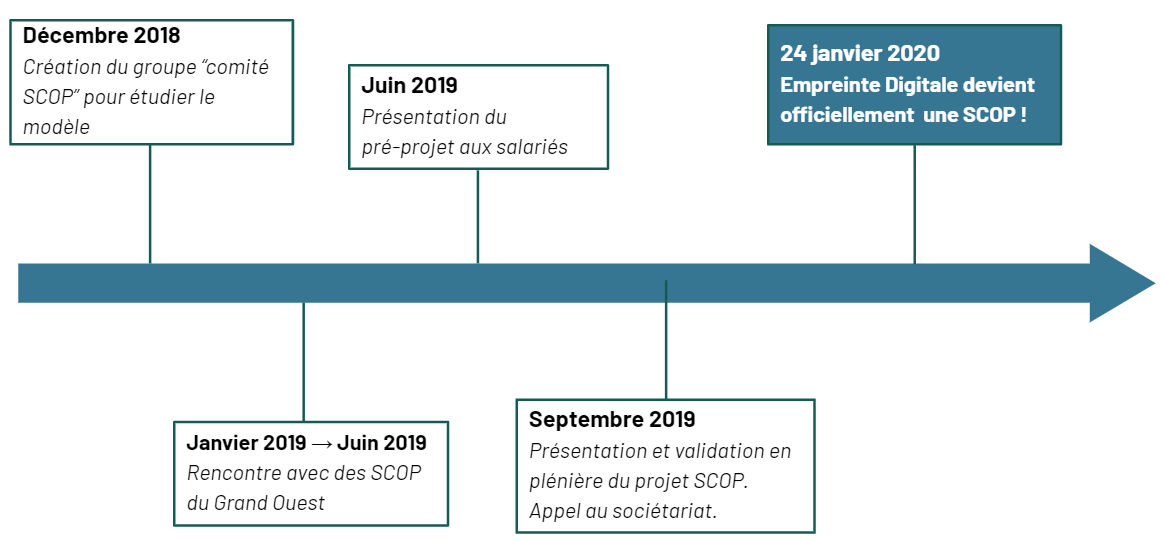
\includegraphics[width=\textwidth]{src/transition_scop.png}
    \caption{Les étapes du passage en SCOP d'Empreinte Digitale}
    \label{fig:transition_scop}
\end{figure}


\newpage
La gouvernance se découpe de la manière suivante :
\begin{figure}[!ht]
    \centering
    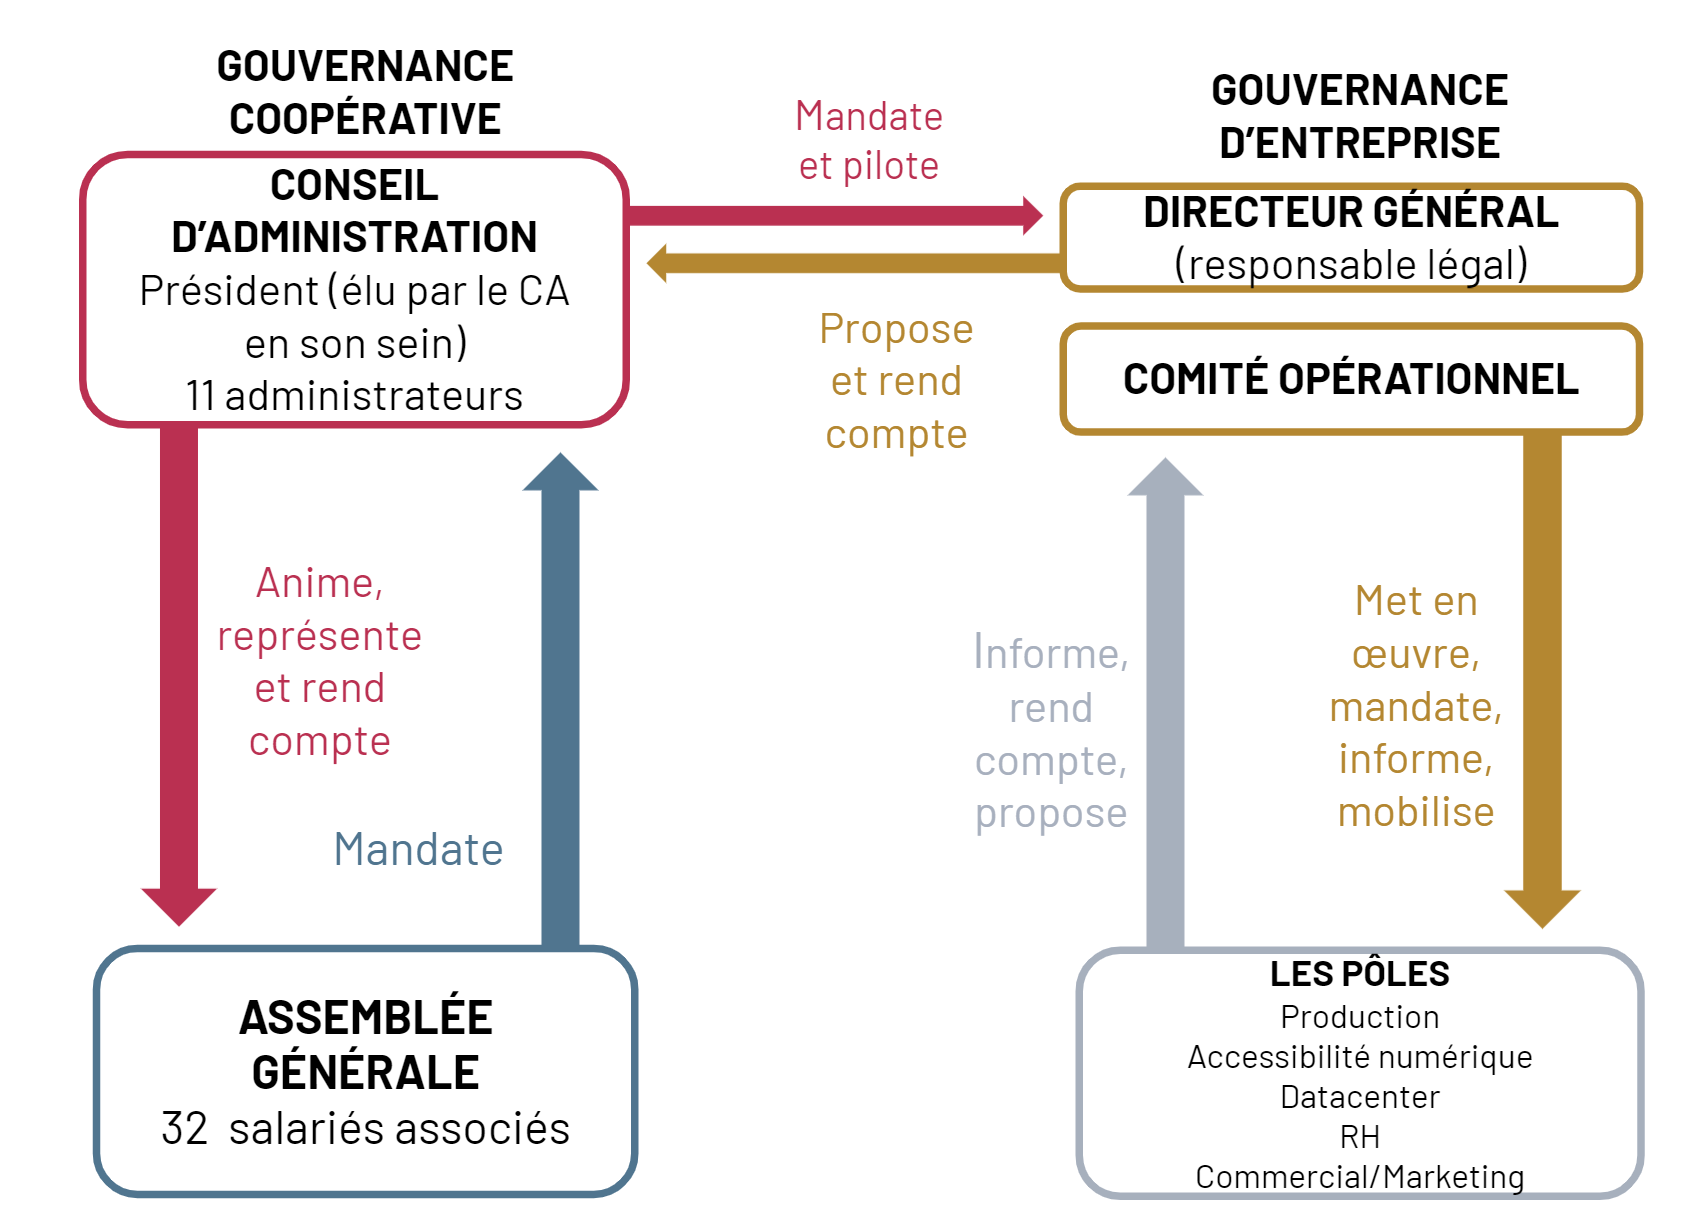
\includegraphics[width=\textwidth]{src/gouvernance_ed.png}
    \caption{Schéma de la gouvernance chez Empreinte Digitale}
    \label{fig:gouvernance_ed}
\end{figure}

La gouvernance coopérative est similaire au fonctionnement d'une association loi 1901 avec les membres de l'association et le conseil d'administration. 
Le conseil d'administration a pour rôle de déterminer les orientations de l'activité de la société. 
Actuellement, l'assemblée générale est consisté de 32 salariés. 
Un salarié ne peut pas rester dans l'entreprise si au bout de 3 ans d'ancienneté celui-ci ne veut pas adhérer à la SCOP. 
Cette assemblée générale mandate le conseil d'administration constitué des membres élus et en "échange", les membres de conseil anime, représente et rend compte aux associés.

De l'autre côté on trouve la gouvernance de l'entreprise, avec un directeur général, responsable légale qui travail avec un comité opérationnel ou COMOP. 
Ils travaillent avec les différents pôles dans la mise en oeuvre de la stratégie d'entreprise.

La partie décisionnel est aux salariés car c'est bien la gouvernance coopérative qui mandate et pilote la gouvernance d'entreprise qui elle propose et rend compte de l'activité.

Une assemblée générale ordinaire à lieu une fois par an pour voter les grandes orientations de l'entreprise, valider les comptes, voter la répartition des bénéfices et également voter pour les nouveaux associées.

\subsubsection{Responsabilité sociétale et environnemental}
L'axe principal de la démarche RSE chez Empreinte Digitale porte sur le numérique responsable, qui intègre à la fois des problématiques environnementales et sociétales.

\noindent%
\begin{minipage}{.7\textwidth}%
Empreinte digitale est officiellement engagés dans une démarche Responsabilité Sociétales des Entreprises (RSE) depuis 2018, année de sa labellisation Lucie ISO 26000. 
LUCIE est une certification qui prouve qu'une entreprise, un produit ou un service à une démarche réussie en matières de RSE.

\end{minipage}%
\hfill
\begin{minipage}{.3\textwidth}%
\begin{center}

\includegraphics[width=0.7\textwidth]{src/lucie.png}
\end{center}
\end{minipage}% \\

Voici quelques projets RSE d'Empreinte Digitale :
\paragraph{Design4Green}
Le Design4Green est un challenge organisé depuis 5 par l'ESAIP, une école d'ingénieur Angevine.
Durant ce hackathon de 48h, les équipes doivent répondre sur un sujet autour de l'éco-conception. 
Le sujet porte chaque année sur la réalisation d'un projet web avec l'obligation de limiter son empreinte environnementale.

En 2021, il fallait développer une interface pour les professionnel de suivi de l'éco-conception d'un projet web intégrant 491 critères.
Empreinte Digitale à participé à cette édition et l'a remporté avec une application statique, éco-conçu et accessible.
Le site est une "Progressive Web App" (PWA), il est alors téléchargé une seule fois et mise en cache dans le navigateur, ainsi il n'y a pas d'aller-retour avec le serveur.

A la clé de ce challenge, un chèque de 1000€ qui fut par la suite placé dans un autre projet RSE, le budget participatif.

\begin{figure}[!ht]
    \centering
    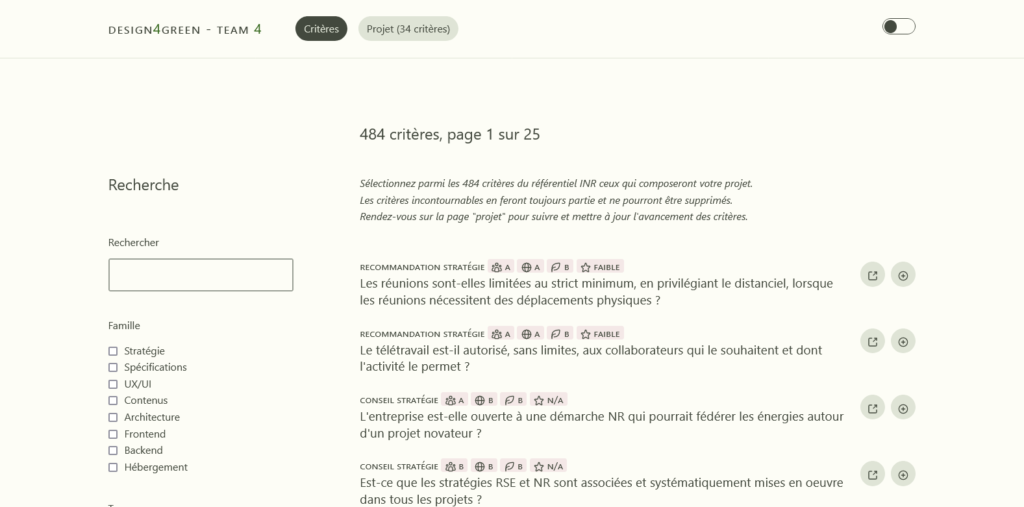
\includegraphics[width=\textwidth]{src/design4fgreen.png}
    \caption{Application web réalisé par Empreinte Digitale pour le Design4Green}
    \label{fig:design4greenl}
\end{figure}

\paragraph{Budget participatif}
En 2022, Empreinte Digitale a lancé un appel à projet nommé Budget Participatif. 
Chaque employé pouvait présenter un ou plusieurs projets qui ont été ensuite soumis à vote. 
Le prix gagné au Design4Green à été mis en jeu et une participation supplémentaire de 1000€ a été attribué par l'entreprise. 
Ainsi, c'est 2000€ de projets, proposés par les salariés, qui ont vu le jours. 
Les proposotions fûrent nombreuses : console de jeu, abri pour oiseaux, salle de sport, jeu de fléchette etc.

\paragraph{Stratosfair}
En 2020, Empreinte Digitale à lancé un partenariat avec Stratosfair. 
L'objectif : créer un datacenter responsable. 
Ce nouveau datacenter à vu le jour deux ans après à Lanester, une ville voisine de Lorient. 
L'idée est d'utiliser des énergies renouvelables produites sur place, la perte d'énergie (chaleur) engendrée par les serveurs et de se "fondre" dans le milieu naturel.
\begin{itemize}
    \item Le datacenter n'est pas posé à même le sol, ne bloquant pas la circulation des organismes vivant.
    \item Une partie de l'énergie qui alimente les serveurs est une énergie renouvelable générée par des panneaux solaires.
    \item La chaleur des serveurs est redirigée dans une serre pour la culture de légumes bio.
\end{itemize}

\begin{figure}[!ht]
    \centering
    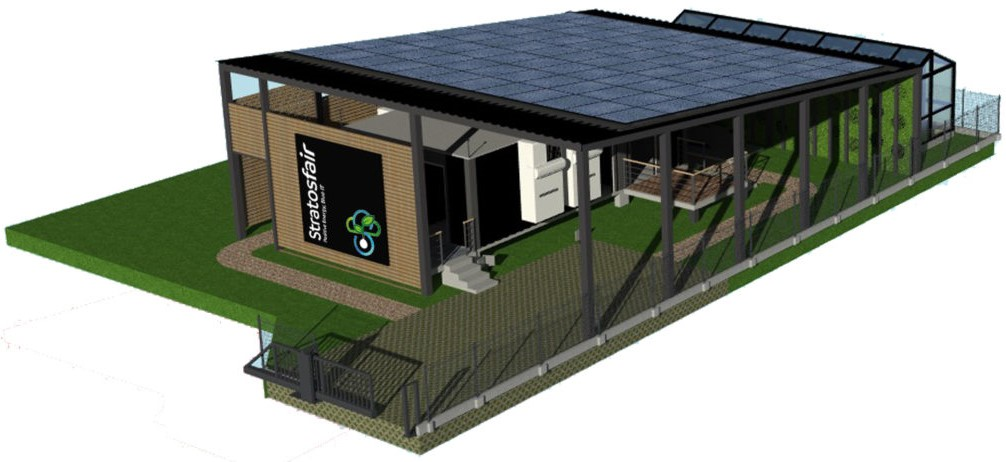
\includegraphics[width=\textwidth]{src/strato.jpg}
    \caption{Maquette 3D du datacenter de Stratosfair}
    \label{fig:strato}
\end{figure}

Avec ce datacenter, Stratosfair et Empreinte Digitale lancent une offre similaire à celle OVH avec la location de machines virtuelles.
Une application et une API ont été développés pour la création de machines virtuelles dans un cluster Proxmox depuis une interface web.

Vous pouvez retrouver d'autres projets RSE ici : \url{https://blog.empreintedigitale.fr}.

\subsubsection{Pôle datacenter}
Empreinte digitale est constitué de 5 pôles : production, accessibilité numérique, datacenter, RH et commercial/marketing.

J'étais intégré dans le pôle datacenter composé de 7 personnes. 
Les activités sont découpeés de la manière suivante :
\begin{itemize}
    \item \textbf{Ligeo} : deux personnes travaillent principalement sur les produits Ligeo. 
    Cela comprend les installations, les mises à jours et la maintenance.
    \item \textbf{Cloud} : une personne travaille sur la conception, les installations et la maintenance des produits cloud. 
    Cela va de l'installation de produits tels que Nextcloud, Zammad, Bitwarden jusqu'à la conception et l'installation d'architecture spécifique à un besoin. 
    C'est le cas par exemple pour le projet Dehon.
    \item \textbf{Travaux interne} : deux personnes, moi y compris, travaillons sur divers travaux interne. 
    Cela concerne notamment les besoins de salariés : PC, mail, comptes, accès, nouveaux outils etc.
    \item \textbf{Commercial} : une personne gère la partie commercial et facturation.
    \item \textbf{Chef de projet} : une personne travaille sur la gestion de projet, en lien avec le commercial.
\end{itemize}

Mise à part la partie commercial et chef de projet, les activités ne sont pas à ce point-là segmentées. 
Dû au astreinte et à l'entre-aide collective, tout le monde "touche à tout". 
Par exemple, bien qu'ayant travaillé majoritairement sur des travaux interne, j'ai également travaillé sur des offres cloud.

\subsubsection{Comité sécurité}
Empreinte Digitale possède un comité sécurité dans lequel j'ai été intégré à mon arrivé.
Celui-ci est composé d'une dizaine de personnes aux profils variés : développeurs, administrateurs systèmes, testeurs et chefs de projet.

Le pôle sécurité étant assez récent, ça mission est pour le moment de maintenir une veille sur la sécurité afin d'apporter des axes d'améliorations. 
Cela tiens compte du développement, de l'hébergement, la documentation et les bonnes pratiques générales à l'attention de tous. 
Le pôle a une réunion hebdomadaire pour suivre l'avancement de divers sujets.

\newpage
\subsection{Sujet}
\subsubsection{Contexte}
Empreinte digitale développe son offre DATACENTER. 
Cela engendre une évolution rapide de l'infrastructure ce qui demande de nouveaux besoins notamment en matière de sécurité. 
En effet, l'entreprise ne possède pas pour le moment d'outils de conformité, d'outils de contrôle de sécurité ni d'outils de \gls{CVE}. 
De plus, il n'y a pas de documentations mis à disposition des salariés afin de spécifier le comportement à avoir lors de l'utilisation du SI ou en cas de faille de sécurité révélée.

\subsubsection{Problématique}
Les problématiques sont multiples :
\begin{itemize}
    \item Comment réaliser un état des lieux du système d'information actuel ?
    \item Comment établir les besoins en hiérarchisant les priorités ?
    \item Comment faire un choix parmi l'ensemble des outils d'audits disponibles ?
    \item Comment pérenniser les solutions mises en oeuvre ? 
\end{itemize}

\subsubsection{Objectifs}
Travailler en mode projet sur l'infrastructure de l'entreprise afin d'améliorer celle-ci en continu. 
Cela passe par la mise en oeuvre de nouveaux outils mais également de nouvelles procédures afin de pérenniser les solutions. 
En parallèle, travailler sur des tâches annexes d'administration système comme installer des plateformes pour les clients, préparer le matériel pour les nouveaux arrivants, etc.

\subsubsection{Outils et ressources}
Les outils sont nombreux et il n'y a pas de restriction à en mettre en oeuvre de nouveaux. 
Les principaux sont ceux cités dans la section \ref{sec: preambule_technique}.

Il n'y a pas de limitation de ressources et matériels.
L'accès aux plateformes vitales à la réalisation des projets est donné avec des droits administrateurs.
Pour les autres plateformes, l'accès est donné ponctuellement lorsque cela est nécessaire et justifié.

L'objectif n'étant pas concentré sur un sujet en particulier, les divers documentations de l'ANSSI servent de conseil.

\newpage
\section{Préambule technique}
\label{sec: preambule_technique}
Les travaux effectués on fait appels à des logiciels régulièrement cités dans ce document. 
Afin de rendre la compréhension de ce rapport plus aisée, cette section décrit brièvement Proxmox, Terraform et Ansible.

\subsection{Proxmox}
\noindent%
\begin{minipage}{.7\textwidth}%
Proxmox est une plate-forme open-source complète pour la virtualisation d'entreprise. 
Grâce à l'interface Web intégrée, nous pouvons facilement gérer les machines virtuelles et les conteneurs, le stockage défini par logiciel, la mise en réseau, le clustering haute disponibilité et plusieurs outils prêts à l'emploi sur une seule solution. \\

\end{minipage}%
\hfill
\begin{minipage}{.3\textwidth}%
\begin{center}

\includegraphics[width=0.5\textwidth]{src/proxmox.JPG}
\end{center}
\end{minipage}% \\

\noindent%
\begin{minipage}{.4\textwidth}%
\begin{center}
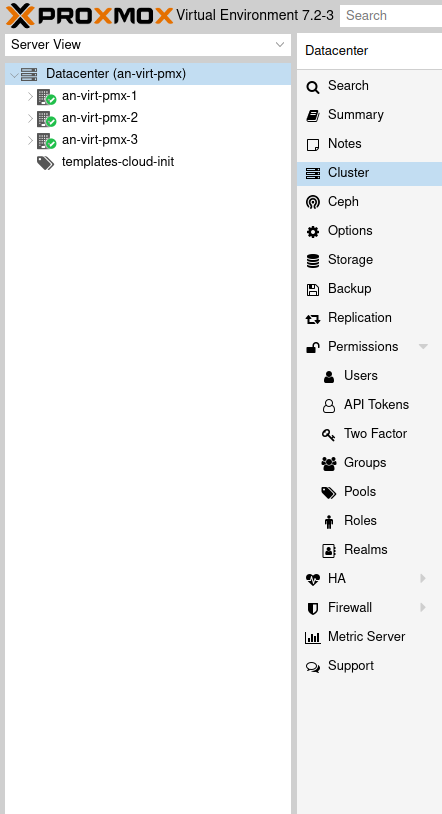
\includegraphics[scale=0.65]{src/proxmox_interface_side.png}
\end{center}

\end{minipage}%
\hfill
\begin{minipage}{.53\textwidth}%
Proxmox possède 3 outils pour manipuler l'ensemble des ressources :
 \begin{itemize}
     \item Un utilitaire en ligne de commande installé.
     \item Une API.
     \item Une interface web.
 \end{itemize}

Depuis l'interface, on visualise l'élément \textit{Datacenter}, correspondant au cluster. 
On visualise également chacun des noeuds du cluster avec leur nom et leur état. 
On peut y modifier les noeuds, les différents stockages, la configuration de backup avec l'ajout de serveur de backup, les permissions utilisateurs, la haute disponibilité du cluster (HA), les statistiques et le support. \\

Il est également possible d'agir sur les machines virtuelles. 
La vision sur les machines virtuelles résume son état, ses caractéristiques telles que l'usage du CPU, de la mémoire, la taille du disque et les adresses IPs. 
On peut y modifier les caractéristiques hardware des machines virtuelles directement à chaud, agir sur le template, accéder à la console de la machine etc. \\
\end{minipage}% \\

\newpage
\subsection{Terraform}
\noindent%
\begin{minipage}{.7\textwidth}%
Terraform est un outil open source d'infrastructure as code développé par Hashicorp. 
Il permet de déclarer sous forme de code l'infrastructure que l'on souhaite obtenir. 
Dans des fichiers de configuration structurés, basé sur un système d'état, on va pouvoir manager l'infrastructure et mettre à jours son état. \\

\end{minipage}%
\hfill
\begin{minipage}{.3\textwidth}%
\begin{center}

\includegraphics[scale=0.5]{src/Terraform.png}
\end{center}
\end{minipage}%

Au travers de scripts dans un langage propre à Terraform, on décrit l'état de l'infrastructure souhaité. 
Son workflow le rend facile à comprendre et à mettre en oeuvre :
\begin{figure}[!ht]
    \centering
    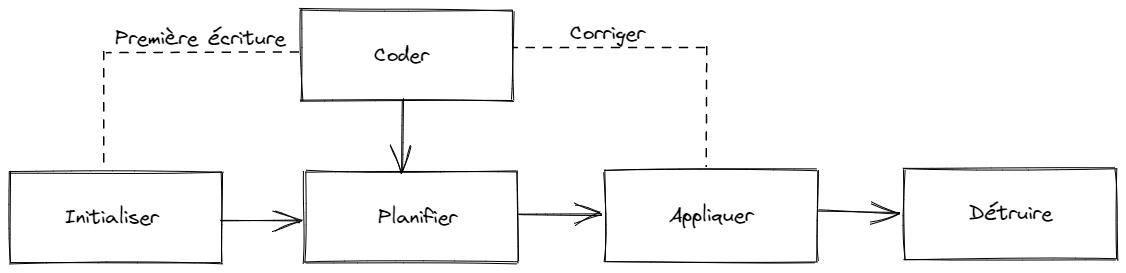
\includegraphics[width=\textwidth]{src/Terraform_schema.png}
    \caption{Workflow de Terraform}
    \label{fig:terraform_schemal}
\end{figure}

Après les quelques première écritures de configuration, on va :
\begin{itemize}
    \item Initialiser le projet avec un nouvel état. Commande : \texttt{terraform init}.
    \item Planifier les configurations. Commande : \texttt{terraform plan}.
    \item Appliquer les configurations. Commande: \texttt{terraform apply}.
    \item Détruire les configurations si nécessaire. Commande : \texttt{terraform destroy}
\end{itemize}

L'étape d'initialisation permet la création d'un état de l'infrastructure qui sera stocké sous la forme d'un fichier \texttt{terraform.tfstate}. 
Cet état permet d'assurer la cohérence entre ce qui est écrit localement et ce qui a déjà été appliqué. 
Dans un travail collaboratif, cette état peut être configuré sur GitLab de façon à assurer la cohérence des états entre différents développeurs.

Terraform se base sur un fonctionnement autour de \textit{providers} ou fournisseurs. 
Un provider est là pour manager une ressource donnée. Ces provider sont nombreux : Amazon Web Services, Google Cloud Plateform, Azure, VmWare Vsphere, Proxmox etc.

A ces providers on spécifie des ressources. 
Chaque bloc de ressources décrit un ou plusieurs objets d'un service. 
La construction d'une ressource est basé sur le provider qui la fournie.

Il est également possible de créer des modules afin de les réutiliser. 
Utile par exemple dans le cas de template de machines virtuelles, où les variables sont toujours les mêmes mais où seuls les valeurs changent.

Chez Empreinte Digitale, Terraform permet le déploiement dans un premier de temps de machines virtuelles sur des cluster Proxmox. 
Par la suite, Terraform permet d'installer des composants sur ces machines telles que des ressources Kubernetes, MongoDB, Helm, etc.

\newpage
\subsection{Ansible}
Nous avons vu précédemment l'intérêt de Terraform dans l'installation de machine de machines virtuelles ou logicielle à partir de différents fournisseurs. 
Une fois cette étapes effectuée, il peut être nécessaire d'effectuer des configuration supplémentaires. 
C'est là qu'Ansible intervient.

\noindent%
\begin{minipage}{.8\textwidth}%
Ansible est un logiciel libre de gestion des configurations qui automatise le déploiement de configurations sur un ensemble de machines. 
Celui-ci est basé sur l'utilisation du protocole SSH. 
Cela lui donne l'avantage de ne pas avoir besoin d'installer d'agents sur les machines, parfois consommateur de ressources.

\end{minipage}%
\hfill
\begin{minipage}{.2\textwidth}%
\begin{center}

\includegraphics[scale=0.3]{src/ansible.png}
\end{center}
\end{minipage}%

Au travers de scripts YAML, on décrit l'état souhaité d'une ou plusieurs ressources pour une ou plusieurs machines. 
Ces scripts vont alors exécuter des modules sur les cibles qui essaieront d'appliquer des correctifs afin d'atteindre cet état souhaité. 
On distingue trois principaux types de scripts :
\begin{itemize}
    \item Les \textbf{rôles}. Ce sont un ensemble de playbooks qui s'assurent de la présence ou absence de fonctionnalité spécifique.
    \item Les \textbf{playbooks}. Ce sont un ensemble de tâches d'automatisations.
    \item Les \textbf{tâches}. Une tâche correspond à la description de l'état souhaité d'un composant d'un machine. 
    Cela peut être exemple la présence ou non d'un paquet apt.
\end{itemize}

L'utilisation de rôle n'est pas toujours nécessaire. 
Un rôle à surtout pour vocation de créer une configuration qui sera réutilisée régulièrement. 
Il donc possible de se limiter à l'utilisation de playbook.

Comme indiqué précédemment, Ansible est dit "agentless". 
Cela signifie qu'il n'est pas nécessaire d'installer d'agents sur les cibles. 
Pour réaliser sa mission, Ansible n'a donc besoin que 3 de pré-requis :  une connexion SSH vers ces cibles, la bonne version de python d'installé sur ces cibles et un inventaire de l'ensemble des cibles.

Lorsqu'un script Ansible est exécuté, la première étape consiste toujours à récupérer les \textit{facts}. 
Ces facts sont l'ensemble des informations de la machine cible. 
On aura le nom de la machine, sa version de système d'exploitation, son numéro de version, etc.

A partir de ces informations on peut paramétrer l'utilisation d'Ansible. 
Cela va notamment permettre de faire une distinction entre les différents systèmes d'exploitation, leurs versions, leurs logiciels installés etc.

Lorsqu'une task Ansible est jouée, il y a 4 états principaux :
\begin{itemize}
    \item \textbf{OK} : la configuration était déjà correcte, Ansible n'a rien changé.
    \item \textbf{SKIPPED} : les conditions d'application de la tâche ne sont pas validées. La tâche est ignorée.
    \item \textbf{CHANGED} : la configuration n'était pas correcte, Ansible à apporté les changements nécessaires avec succès.
    \item \textbf{ERROR} : la configuration ne s'est pas bien passé, Ansible renvoit l'erreur associée.
\end{itemize}

\newpage
\section{Travaux de sécurité}
\subsection{Période d'alternance}
Mon sujet \textbf{Analyse et réalisation d'audits automatisés de l'infrastructure} s'est découpé en 4 phases :

\begin{enumerate}
    \item \textbf{Analyse abstraite et bonnes pratiques}. J'ai réalisé une veille technologique sur les logiciels et outils utilisés par les administrateurs systèmes. 
    De plus, j'ai pris le temps de me cultiver sur les sujets de sécurité avec les documentations et livres blanc de sécurité de l'ANSSI ainsi que les sites de conseils de sécurité sur Internet.
    \item \textbf{Analyse}. J'ai débuté une analyse de l'infrastructure en me basant sur les critères du référentiel secNumCloud de l'ANSSI. 
    Cette analyse n'était pas uniquement technique car parmi les critères de certification, de nombreux points concernent de la documentation.
    \item \textbf{Préconisations}. J'ai rédigé des documentations pour le pôle \gls{sysadmin} et l'ensemble des salariées : livre blanc de sécurité, PSSI (Plan de sécurité des systèmes d'information), etc.
    \item \textbf{Mise en oeuvre}. J'ai effectué des \gls{POC} sur Rudder et Ansible CMDB.
\end{enumerate}

A l'issue de mes travaux, j'ai rédigé un PSSI et un tableau de suivi d'audit de l'infrastructure. 
Les deux documents sont composés de 16 thématiques présentés en annexe de ce document aux pages \pageref{tab:16thematiques1} et \pageref{tab:16thematiques2}.
\begin{figure}[!ht]
    \centering
    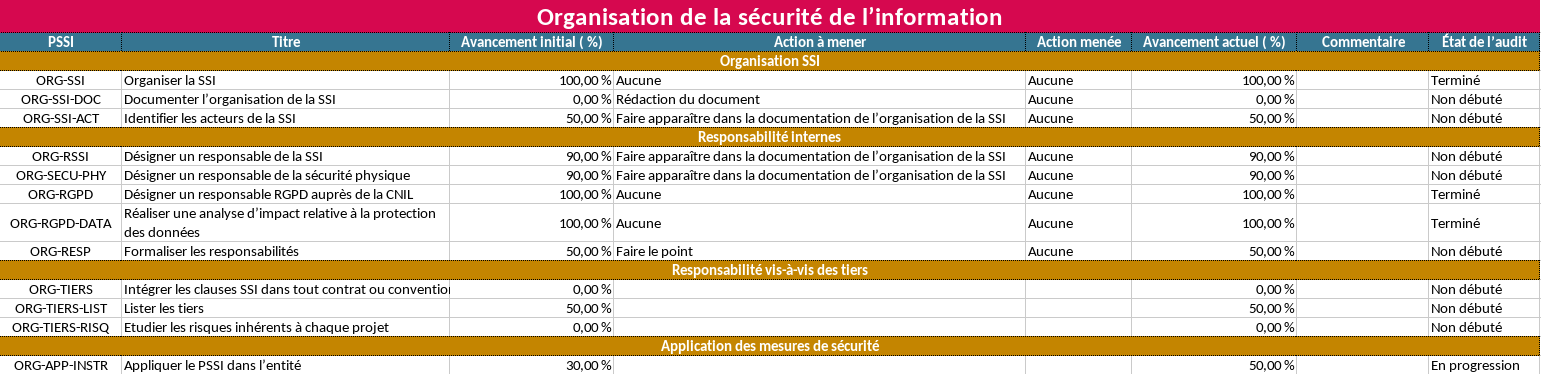
\includegraphics[width=\textwidth]{src/table_example.png}
    \label{fig:pssi_table}
    \caption{Extrait du tableau de suivi de sécurité}
\end{figure}

J'ai par la suite complété ce tableau afin de mettre en avant les points déjà mis en oeuvre au sein et ceux qui ne l'était pas.

\newpage
\subsection{Inventaire des machines}
\subsubsection{Description}

Dans le cadre de la 4\textsuperscript{ème} thématique portant sur la gestion des actifs, il est nécessaire de tenir un inventaire des ressources informatiques. 
Cela comprend l'ensemble des ordinateurs du personnel, les machines physiques liées au différents datacenters ainsi que les machines virtuelles qu'elles hébergent.
La solution retenue est d'utiliser 2 logiciels open-source :

\noindent%
\begin{minipage}{.7\textwidth}%
\textbf{Open Computers and Software Inventory (OCSInventory)} une solution open-source de gestion technique de parc informatique. 
Ce logiciel libre permet l’inventaire hardware et software. 
On va ainsi inventorier des machines avec leurs caractéristiques matériels et les logiciels qui y sont installés.
\end{minipage}%
\hfill
\begin{minipage}{.3\textwidth}%
\begin{center}

\includegraphics[width=0.7\textwidth]{src/logo_ocsinventory.png}
\end{center}
\end{minipage}% \\

\noindent%
\begin{minipage}{.7\textwidth}%
\textbf{Gestionnaire Libre de Parc Informatique (GLPI)} est une solution open-source de gestion de parc informatique qui permet la classification des différentes ressources. 
Ce logiciel libre permet l’inventaire hardware et software. 
On va ainsi inventorier des machines avec leurs caractéristiques matériels et les logiciels qui y sont installés.
\end{minipage}%
\hfill
\begin{minipage}{.3\textwidth}%
\begin{center}

\includegraphics[width=0.7\textwidth]{src/logo_glpi.png}
\end{center}
\end{minipage}% \\

OCSInventory va permettre de récupérer les informations tandis que GLPI va les trier en fonction de règles.

\subsubsection{Architecture}
\begin{figure}[!ht]
    \centering
    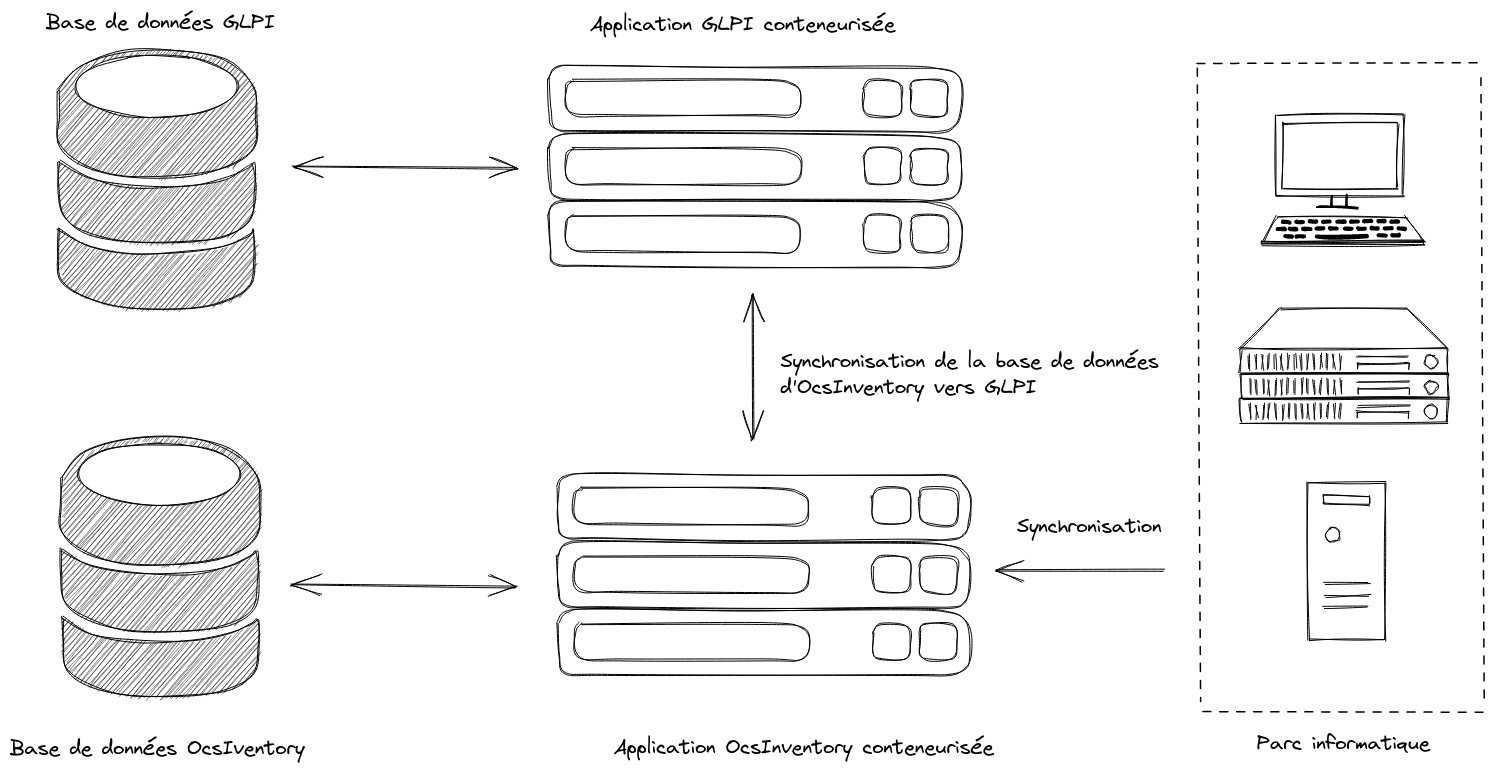
\includegraphics[width=\textwidth]{src/Fonctionne GLPI.png}
    \label{fig:glpi}
    \caption{Architecture entre OcsInventory et GLPI}
\end{figure}

\newpage
\subsubsection{Principe de fonctionnement}
L'application OCSInventory fonctionne sur un système d'agent.
C'est-à-dire qu'un agent est installé sur l'ensemble des machines, et celui-ci va par la suite envoyer des rapports quotidiennement via le protocole HTTP au serveur maître. 

Ensuite, l'application GLPI avec un plugin dédié à l'import des données d'OCSInventory va se connecter à l'application OCSInventory et lire les données.
Finalement, par une action manuelle à réaliser dans GLPI, je valide les imports.

L'agent est paramétré avec un champ TAG avec les critères suivants :
\begin{itemize}
    \item \textbf{ANG-ORD} : ordinateurs des salariés d'Angers.
    \item \textbf{ANG-DC} : serveurs physiques et machines virtuelles d'Angers.
    \item \textbf{REN} : serveurs physiques et machines virtuelles de Rennes.
    \item \textbf{TRS} : serveurs physiques et machines virtuelles de Tours.
\end{itemize}

Une fois l'import fait, je peux dans GLPI visualiser les machines avec les TAGs associés. 
Le TAG va alors permettre de tirer lors de l'import l'affectation dans des \textit{organisations} basées sur la localisation.
Lorsqu'un import est validé, GLPI écrit dans une base de données qui lui ait propre les informations.

Une autre architecture aurait été possible en utilisant FusionInventory à la place d'OCSInventory. 
L'avantage de FusionInventory est qu'il ne possède pas sa propre base de données. 
Une fois les données récupérées, il les inscrit directement dans la base de données de GLPI. 
Cette solution n'a pas été retenue car un serveur OCSInventory était déjà utilisé.

\subsubsection{Serveur maitre}
Le serveur maitre de d'OCSInventory est installé dans un conteneur dans le cluster Proxmox d'Angers.
Je n'ai pas eu à installer cette partie, l'application existait déjà.

J'ai installé GLPI avec Docker sur une machine dédié aux conteneurs.

\subsubsection{Ajout d'un plugin}
Par défaut, OCSInventory ne possède pas de plugin permettant d'inventorier les vhosts. 
Les vhosts sont les noms des sites webs hébergés sur une machine et il est intéréssant de pouvoir déterminer sur quelle machine est installé un site. 
Afin de répondre à ce besoin interne, j'ai repris le travail d'un collègue avec l'écriture d'un script Perl permettant d'inventorier les vhosts des serveurs web Nginx, des conteneurs Docker et de les écrires dans la base de données d'OCSInventory.
Le nom des sites ayant une structure comprenant à la fois le service et le nom du client, il est possible de faire du traitement afin de créer une nouvelle table spécifiquement pour le nom des clients.
Cela se fait pas un traitement du même résultat que pour les vhost.

\subsubsection{Installation et configuration avec Ansible}
\paragraph{Bastion SSH}
L'une des problématiques du projet est d'installer les agents sur chacune des machines du SI. 
Cela représente environ 700 machines virtuelles. 
Heureusement, l'accès aux différentes machines passe par un Bastion SSH. 
Cela fonctionne par un contrôle d'accès basé sur les rôles (RBAC). 
Le rôle \textit{sysadmin} dont je fais partie donne les droits sur toutes les machines. 
La machine Passhport permet d'avoir un accès SSH à l'ensemble des machines virtuelles.
C'est donc par cette machine que les scripts Ansible seront exécutés.

\paragraph{Inventaire}
Ansible se base sur des fichiers d'inventaire dans lequel on décrit le nom des machines dans différents niveaux de catégories. 
La première chose que j'ai fais est de mettre à jours l'inventaire. 
En effet, la différence de nombre de machines entre le Bastion SSH et l'inventaire Ansible mettait en avant qu'il en manquait au niveau d'Ansible. 
J'ai alors fais une comparaison entre le listing du Bastion et celui d'Ansible pour en ressortir les machines manquantes.

Ensuite j'ai repris la structure de l'inventaire. 
Parmi les différents groupes de celui-ci, il y a 3 groupes permettant de distinguer les machines se trouvant sur Angers, Rennes et Tours. 
Cependant, après avoir visualisé l'inventaire sous forme d'arborescence avec la commande \verb|ansible-inventory|, j'ai remarqué qu'il y avait des petites erreurs. 
J'ai corrigé ces erreurs petit à petit en me basant sur la représentation de l'inventaire sous forme de graphique.

\paragraph{Rôle Ansible}
Un rôle est découpé de la manière suivante :
\begin{verbatim}
|-- ocsinventory-agent
|   |-- /default            # Variables par défaut
|   |-- /files              # Fichiers supplémentaires
|   |-- /meta               # Nécessaire pour d'Ansible Galaxy
|   |-- /tasks              # Ensemble des playbooks
|   |-- /vars               # Fichier de variables supplémentaires
\end{verbatim}

\begin{itemize}
    \item \textbf{Default} : variables pour le TAG, le nom des paquets, etc.
    \item \textbf{Files} : scripts supplémentaire d'installation du plugin.
    \item \textbf{Meta} : enregistrement du créateur du rôle. Ce dossier est nécessaire pour utiliser Ansible-Galaxy.
    \item \textbf{Tasks} : ensemble des tâches Ansibles.
    \item \textbf{Vars} : variables supplémentaires s'il est nécessaire de modifier les valeurs pas défaut.
\end{itemize}

\newpage
Le diagramme de séquence ci-dessous met en lumière de façon simplifié les différentes tâches Ansible. On considère que l'ensemble des tâches se sont déroulés sans erreurs.

\begin{figure}[!ht]
    \centering
    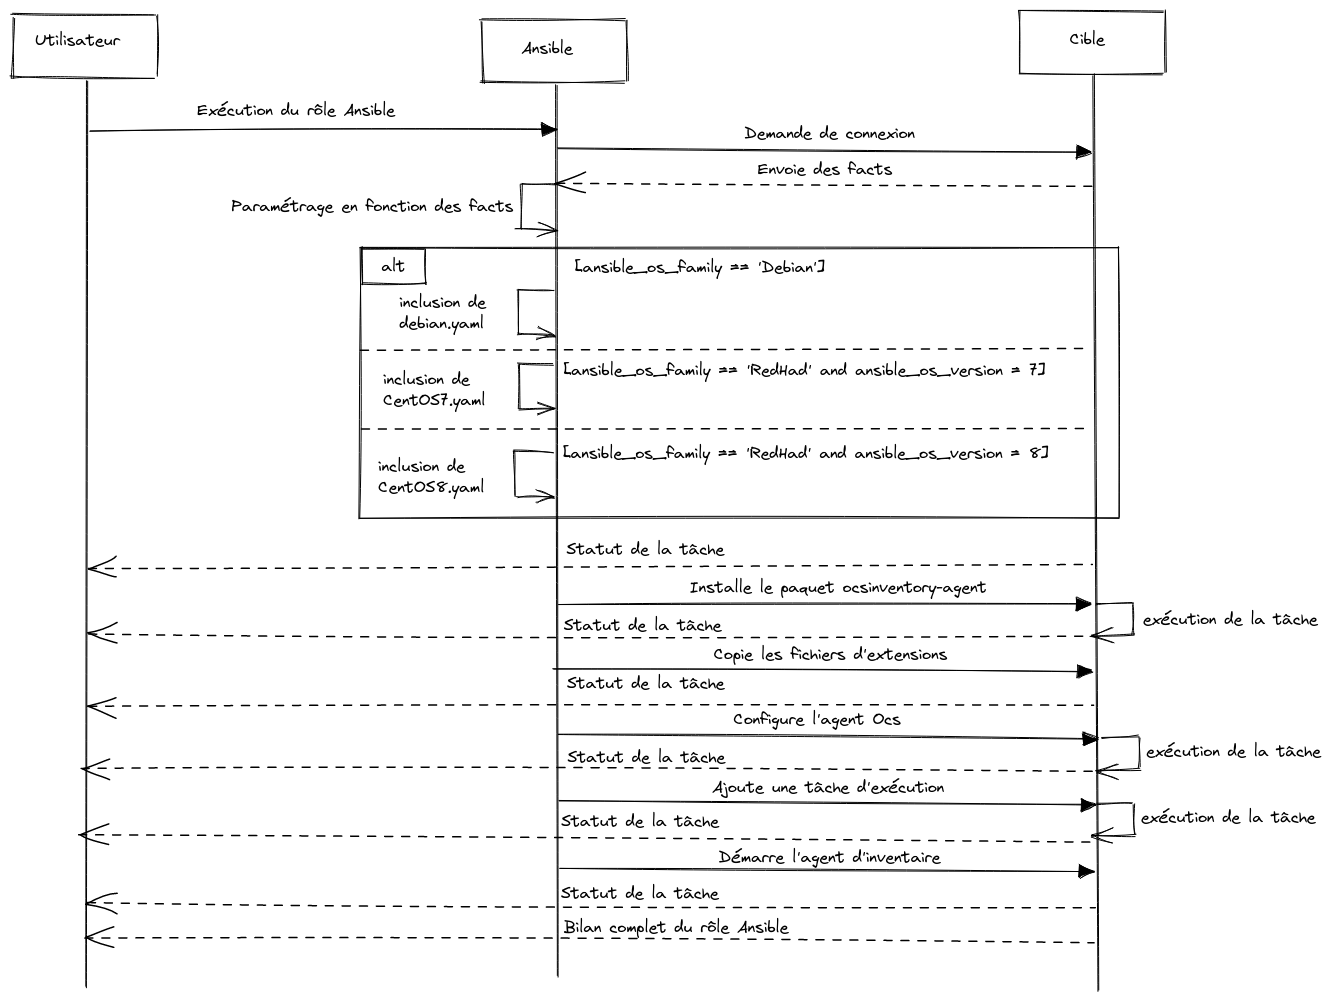
\includegraphics[width=\textwidth]{src/Ansible OCS.png}
    \label{fig:ansible_ocs}
    \caption{Diagramme de séquence de l'installation d'OCSInventory avec Ansible}
\end{figure}

L'utilisateur exécute le rôle Ansible.
Cela va lancer une série d'étapes durant lesquelles Ansible va se connecter en SSH à la cible.
Dans un soucis de simplicité, on considère ici que la connexion est acceptée et Ansible récupère l'ensemble des facts.
A lieu ensuite un paramétrage dépendant des facts. 
Dans le cas de cette installation d'OCSInventory, cela prend en compte la famille du systèmes d'exploitation et sa version.
A l'issues de ces étapes, divers tâches vont permettre l'installation et la configuration de l'agent sur la cible.

Afin que les salariés installent pas eux-même l'agent, j'ai rédigé une documentation décrivant comment installer et configurer l'agent OCSInventory sur Windows, Linux et ArchLinux.
\newpage
\subsubsection{Bilan}
L'installation sur les machines accessibles via le réseau d'Angers est terminée.
L'ensemble des salariés ont également installé l'agent.
L'agent est installé sur la majorité des machines du datacenter de Rennes.
L'agent est installé sur les machines de Tours. 
Cependant, le réseau d'Angers et Tours n'étant pas encore relié à la date de ces installations, les agents ne peuvent pas joindre le serveur OCSInventory.

\newpage
\subsection{Durcissement Linux}
\subsubsection{Objectif}
Dans le cadre de la 8\textsuperscript{ème} thématique portant sur la sécurité liée à l'exploitation, il est nécessaire d'effectuer un durcissement des systèmes Linux à l'installation d'une nouvelle machine. 
En effet, une machine installée à partir de l'image d'origine n'est pas suffisamment sécurisée.

Pour répondre à ce besoin, j'ai décidé d'utiliser OpenSCAP et Ansible. 
L'objectif est d'utiliser les fonctionnalité d'OpenSCAP en les automatisant avec Ansible.
Je cherche à obtenir pour chaque machine un rapport initial, le script Ansible de correctif et un rapport finale après application des correctifs. 

\subsubsection{Openscap}
\noindent%
\begin{minipage}{.7\textwidth}%
OpenSCAP représente à la fois une bibliothèque et un outil de ligne de commande qui peuvent être utilisés pour analyser et évaluer chaque composant de la norme SCAP. 
L'outil de ligne de commande, appelé oscap, offre un outil polyvalent conçu pour formater le contenu en documents ou analyser le système en fonction de ce contenu. \\
\end{minipage}%
\hfill
\begin{minipage}{.3\textwidth}%
\begin{center}

\includegraphics[width=0.8\textwidth]{src/logo_openscap.png}
\end{center}
\end{minipage}%

Egalement, il permet d'effectuer un scan d'une machine et de générer un rapport HTML.
Depuis ce même rapport, il est possible de générer une ensemble de tâches Ansible corrigeant les erreurs.

\subsubsection{Création de machines virtuelles de test}
Avant de procéder à l'installation et l'exécution d'Openscap sur l'ensemble des machines, il est nécessaire de le tester. En effet, l'outil effectuant de nombreuses modifications à la volé, il faut d'abord éprouver la solution afin de s'assurer qu'elle n'entraîne pas de modifications handicapent pour l'exploitation.
Ainsi, afin d'avoir un panel assez large pour effectuer des tests, j'ai créé sur le Proxmox d'Angers 6 machines virtuelles :
\begin{table}[ht!]
    \begin{center}
        \begin{tabular}{| c | c | c | c | c |}
        \hline
        Nom de la distribution & Version & Espace disque & CPU & Ram 
        \tabularnewline

        \hline
        Debian & 10 & 32 Gb & 2 & 2 Gb
        \tabularnewline

        \hline
        Debian & 11 & 32 Gb & 2 & 2 Gb
        \tabularnewline

        \hline
        Ubuntu & 20.04 & 32 Gb & 2 & 2 Gb
        \tabularnewline

        \hline
        Fedora & 36 & 32 Gb & 2 & 2 Gb
        \tabularnewline

        \hline
        Centos & 7 & 32 Gb & 2 & 2 Gb
        \tabularnewline

        \hline
        Centos & 8 & 32 Gb & 2 & 2 Gb
        \tabularnewline
        \hline
        \end{tabular}
    \end{center}
    \caption{Machines virtuelles créés pour les tests avec OpenSCAP}
\end{table}

\subsubsection{Création d'une archive Debian}
Le paquet ne se trouve pas dans les listes des sources apt de Debian 11. 
J'ai débuté la création de l'archive Debian à partir des sources du paquet mais je n'ai pas réussi pour le moment.

\subsubsection{Installation et configuration avec Ansible}
A nouveau, c'est avec Ansible que la configuration d'Openscap est faite. 
Le diagramme de séquence suivant décrit le processus d'installation. 
Afin de le simplifier, la différenciation entre distribution et version n'est pas représentée.

\begin{figure}[!ht]
    \centering
    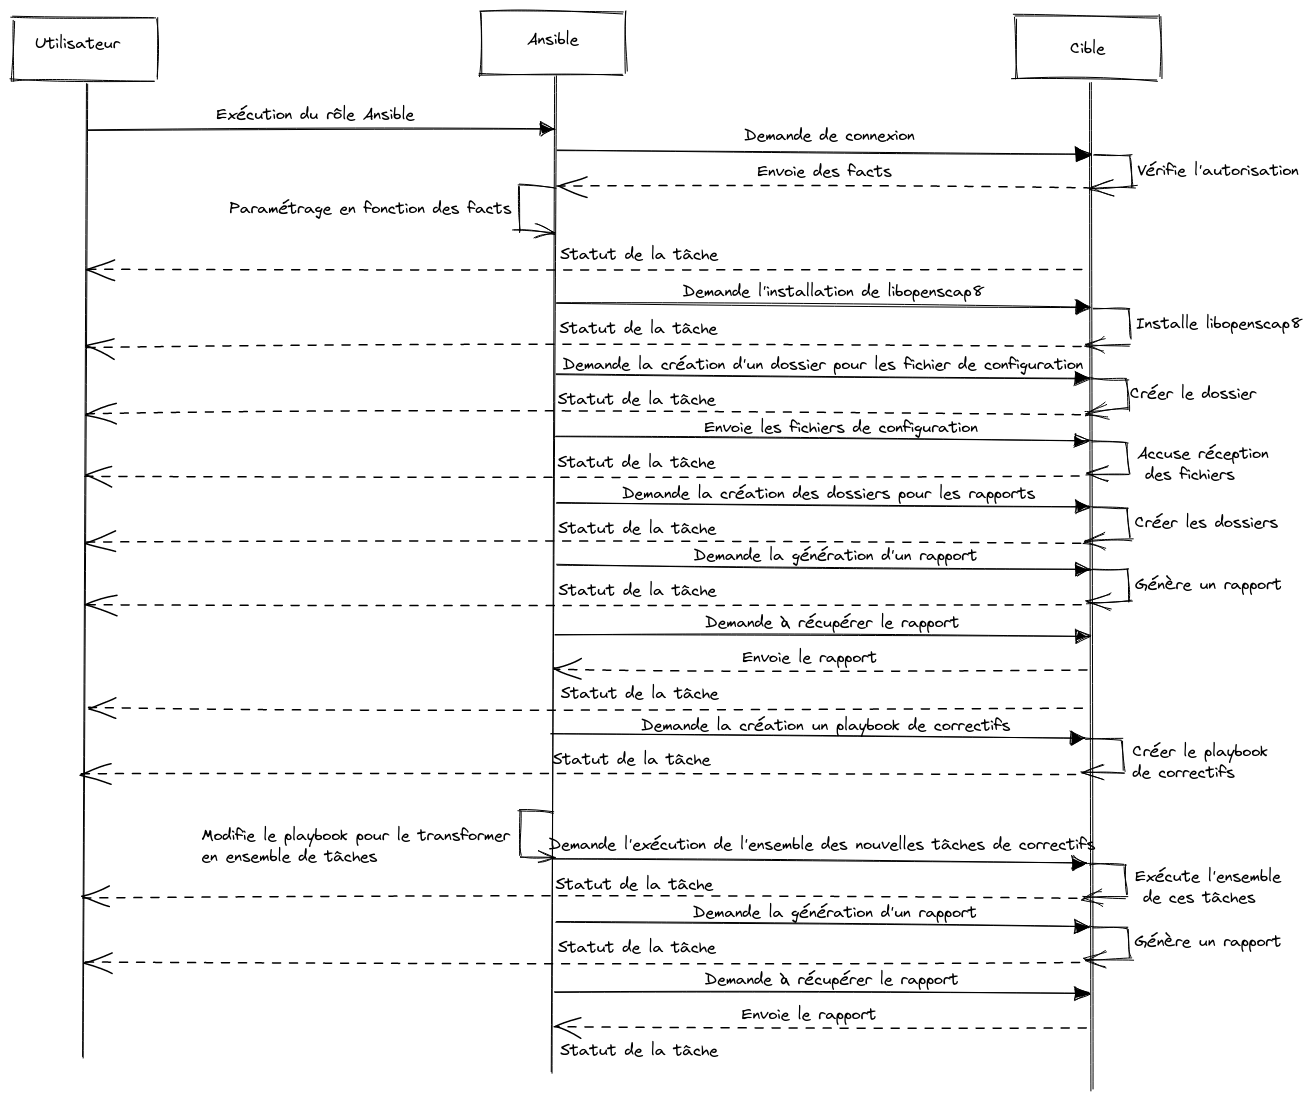
\includegraphics[width=\textwidth]{src/Ansible oscap.png}
    \label{fig:ansible_oscap}
    \caption{Diagramme de séquence du fonctionnement d'Ansible avec OpenSCAP}
\end{figure}

\newpage
\subsubsection{Bilan}
Au moment de la rédaction de ce rapport, l'installation et l'exécution d'Openscap n'a pas été réalisée sur l'ensemble des machines. 
Cependant l'ensemble des tests en fonction des distributions est fonctionnel.
En l'état, l'outil est intéressant. 
Il ne peut pour autant pas être mis oeuvre tel quel car certaines règles sont trop restrictives.
Par exemple, une des modifications apportées avec OpenSCAP fait que la connexion SSH à l'utilisateur root est désactivée.
Cependant, lorsque l'on passe par le bastion SSH, toutes les connexions se font sur l'utilisateur root.
Appliqué la script en l'état empêcherait l'utilisation du bastion.

\newpage
\subsection{Documentation}
\subsubsection{Objectif}
Dans plusieurs des thématiques portant sur la sécurité, un aspect documentaire est mis en avant. 
Il s'agit d'avoir des documents descriptifs de l'infrastructure, de procédures et processus liés à l'exploitation ou de documents juridiques sur les engagements qui doivent être mis en oeuvre entre employeur et salariés, mais aussi clients et prestataire. 
L'objectif est d'avancer sur les documentations manquantes et d'établir un fonctionnement afin d'en assurer la pérennité.

\subsubsection{Documents}
Lors de l'alternance j'ai travaillé sur la Politique de Sécurité des Systèmes d'Information (PSSI) ainsi que sur la charte informatique. 
Durant la période de stage, j'ai travaillé sur la reprise de la documentation interne du datacenter afin de rédiger surtout les procédures, politiques et processus déjà mis en oeuvre mais dont il manquait l'aspect documentaire.
De plus, suite à la demande d'un client, j'ai rédigé un Plan d'Assurance Sécurité (PSA) spécifiant les devoirs entre prestataires et clients au niveau de l'exploitation des services installés par Empreinte Digitale.

\subsubsection{Outils}

\noindent%
\begin{minipage}{.7\textwidth}%
La documentation à destination des clients et prestataire est rédigée soit sur le Google Drive soit sur le Nextcloud de l'entreprise. 
Quant aux documentations internes au Sysadmin ou à l'ensemble des salariés, celles-ci sont rédigés sur un Wiki.js, une application open-source hébergée en interne. 
Cette application permet de rédiger des documents en markdown depuis une interface web.

\end{minipage}%
\hfill
\begin{minipage}{.3\textwidth}%
\begin{center}

\includegraphics[width=.6\textwidth]{src/wikijs.jpeg}
\end{center}
\end{minipage}%

\subsubsection{Bilan}
Il reste encore de nombreuses documentation à rédiger et notamment de la documentation qui nécessite la mise en place de révision annuelle.
Bilan en temps :


\newpage
\subsection{Autres pistes d'étude}
Les outils présentés précédemment ont été mis en application sur l'ensemble du système d'information. 
Cependant, d'autres essaies ont été fait.

Durant la période de d'alternance, j'ai fais des essaies avec Ansible CMDB. Cette solution bien que non retenue pourrait être reconsidérer. 
Son aspect ne nécessitant qu'une connexion SSH permet de gérer la totalité du parc, contrairement à d'autres comme OcsInventory qui posait des problèmes liés au réseau.

J'ai également testé Rudder durant l'alternance. 
Techniquement, la solution est intéressante mais possède un coût important.

Wazuh une plate-forme gratuite et opensource de sécurité basé sur un fonctionnement d'agent était également intéressante. 
Celle-ci permet de réaliser du monitoring de sécurité ainsi que de l'application de correctifs. reposant sur ElasticSearch et Kinana, l'interface web paramétrable permet une excellente vision de l'ensemble du SI en temps réel. 
Néanmoins, le fonctionnement par agent est contraignent et la configuration uniquement via des fichiers XML rend le travail fastidieux.

Enfin, OpenVas un outils opensource de scan de vulnérabilités de site WEB permet de générer des rapports sur un nombre illimité de sites. 
Je ne suis pas aller très loin dans l'expérimentation avec mais elle mériterait de passer plus de temps d'expérimentation.

\newpage
\subsection{Bilan}


\newpage
\section{Travaux d'administrateur système}
\subsection{Nextcloud et Collabora}
\noindent%
\begin{minipage}{.7\textwidth}%
Nextcloud est une application web libre d'hébergement de fichiers et une plateforme de collaboration. 
Associé à Collabora, une suite bureautique, il est possible d'intégrer dans Nextcloud l'édition de fichiers en tout genre de façon Collaborative. 
Cette suite logiciel est finalement une alternative libre et open-source à l'utilisation d'outils tels que Google Drive ou OneDrive.
\end{minipage}%
\hfill
\begin{minipage}{.3\textwidth}%
\begin{center}

\includegraphics[width=0.5\textwidth]{src/nextcloud.jpeg}
\end{center}
\end{minipage}% \\

\subsubsection{Objectif}
Empreinte Digitale installe et héberge régulièrement des instances Nextcloud et Collabora. 
L'objectif est de simplifier et automatiser au mieux les installations mais également de facilité les mises à jours.

Pour répondre à ces besoins, 4 outils sont utilisés :
\begin{itemize}
    \item \textbf{GitLab} pour stocker l'ensemble des ressources nécessaires à l'installation.
    \item \textbf{Ansible} pour exécuter différentes tâches.
    \item \textbf{Ansible Tower/AWX} pour gérer depuis une interface graphique l'application des tâches Ansible et assurer un maintien dans le temps.
    \item et \textbf{Jinja} couplé à Ansible pour permettre de générer les fichiers de configurations avec les bonnes variables en se basant sur des templates.
\end{itemize}

\subsubsection{Description}
L'application repose sur des conteneurs Docker hébergés sur une machine virtuelle, elle-même dans un cluster Promox. On compte 5 composants :
\begin{itemize}
    \item \textbf{Nextcloud} notre application principale associée à un serveur web apache dans un unique conteneur.
    \item \textbf{Collabora} l'application supplémentaire pour l'édition de texte.
    \item \textbf{Traefik} le reverse proxy qui va exposer les sites web \verb| collabora.cloud-ed.fr | et  \verb| nextcloud.cloud-ed.fr|. 
    C'est également au niveau de Traefik que sont gérés les certificats HTTPs.
    \item Une base de donnée \textbf{PostgreSQL} pour l'applicatif.
    \item Un cache applicatif \textbf{Redis}.
\end{itemize}

\newpage
\subsubsection{Schéma applicatif}
\begin{figure}[!ht]
    \centering
    
\includegraphics[width=0.7\textwidth]{src/Nextcloud stack.png}
    \caption{Schéma applicatif de Nextcloud avec Collabora}
    \label{fig:nextcloudXcollabora}
\end{figure}

\subsubsection{Utilisation des variables}
Automatiser aux mieux l'installation revient à créer un "Template" d'installation, n'utilisant que des variables. 
On distingue 2 types de variables :
\begin{itemize}
    \item \textbf{Les variables d'environnements}. Celles-ci vont décrire le nom du client, la version de Nextcloud à installer, les images Docker à utiliser etc. 
    Ce sont les variables qui n'ont pas besoin d'êtres secrètes.
    \item \textbf{Les secrets}. Ce sont d'autres variables obligatoires sauf qu'elles sont sensibles et donc à protéger. 
    C'est le cas notamment des identifiant et mots de passes des services.
\end{itemize}

Les variables sont utilisées à 3 endroits différents :
\begin{itemize}
    \item Dans les fichiers docker-compose, qui prennent leurs valeurs dans le fichier \verb|.env|.
    \item Dans le fichier \verb|.env|, qui est généré depuis Ansible avec un template Jinja.
    \item Dans le template Jinja, qui prend ses valeurs dans l'\verb|inventory| AWX et également dans le coffre-fort Ansible.
\end{itemize}

La personne qui réalise l'installation doit spécifier les variables dans l'\verb|inventory| AWX et dans le coffre-fort Ansible.

Finalement, à partir d'un template Jinja et d'Ansible, on génère un fichier \verb|.env| que l'on place dans le dossier de l'application Nextcloud afin qu'il soit utilisé par les scripts docker-compose.

\subsubsection{Inventaire Ansible}
Le paramétrage des variables pour le rôle et le vault est la première étape. 
Ensuite, il faut mettre à jours l'inventaire Ansible du rôle. Dans le dépôt GitLab dans lequel se trouve le playbook générique, un dossier \verb|group_vars| permet de distinguer les différentes vaults.
Par exemple :
\begin{verbatim}
|-- group_vars
|   |-- aicla               # Vault du client aicla
|   |   |-- vault.yaml
|   |-- ed                  # Vault du client ed
|       |--vault.yaml
\end{verbatim}

Pour appliquer correctement le vault pour aicla et ed, il faut créer un groupe dans l'inventaire Ansible portant le même nom. 
Le fichier \verb|host| contient :
\begin{verbatim}
[aicla]
aicla-cloud-1 ansible_host=192.168.X.X

[test]
an-nextcloud-test ansible_host=192.168.X.X
\end{verbatim}

Il faut comprendre que le groupe \verb|aicla| possède une machine nommée \verb|aicla-cloud-1| dont l'adresse IP est \verb|192.168.X.X|. 
Ce groupe possède des variables de groupe, d'où le nom \verb|group_vars|, spécifié dans le fichier \verb|group_vars/vault.yaml|.

\subsubsection{Utilisation d'AWX}
Une fois l'inventaire et les variables mis à jour, il faut paramétrer AXW. Tout se fait par le biais d'une interface web comme ci-dessous :
\begin{figure}[!ht]
    \centering
    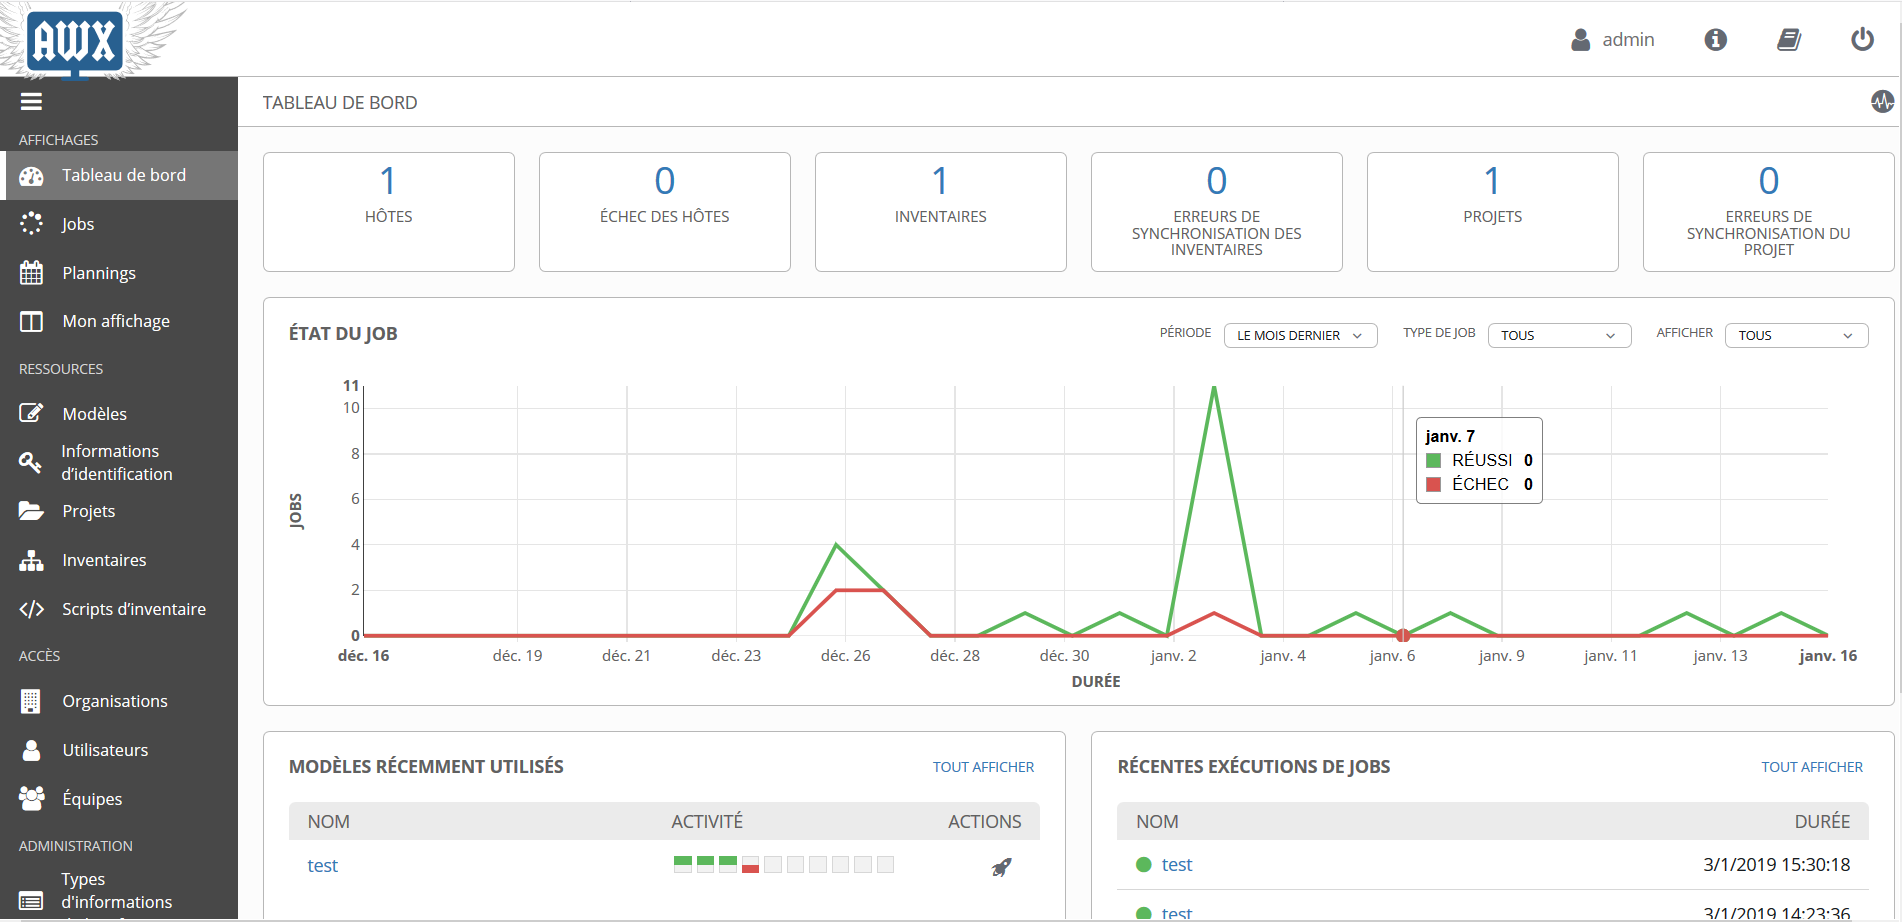
\includegraphics[width=\textwidth]{src/awx.png}
    \caption{Interface web d'AWX}
    \label{fig:awx}
\end{figure}

Dans AWX, j'ai créé un projet \verb|Nextcloud|. 
Dans ce projet, je fais appel à une source \verb|Git| qui est mon dépôt GitLab avec le nom de la branche et les identifiants à utiliser. 
Le principe est que ce projet n'est pas à être changer.

Ensuite je créer un \verb|Template|, utilisant mon projet \verb|Nextcloud| et d'autres ressources. 
Les ressources supplémentaires à créer sont :
\begin{enumerate}
    \item Inventaires : variables d'environnement. 
    \item Script d'inventaire : nom de la machine et son adresse IP.
    \item Informations d'identification : accès au dépôt GitLab et mot de passe du Vault Ansible.
    \item Modèles : spécifier l'utilisation des éléments précédemment créé, c'est-à-dire l'inventory, l'host, les credentials et le projet Nextcloud.
\end{enumerate}

\subsubsection{Rôle Ansible}
Le schéma ci-dessous décrit les actions réalisées par le rôle Ansible appelé par Ansible AWX. 
Celui-ci ne fait pas apparaître les différentes tâches liés aux dépendances tels que l'installation du module \verb|pip| pour Python.

\begin{figure}[!ht]
    \centering
    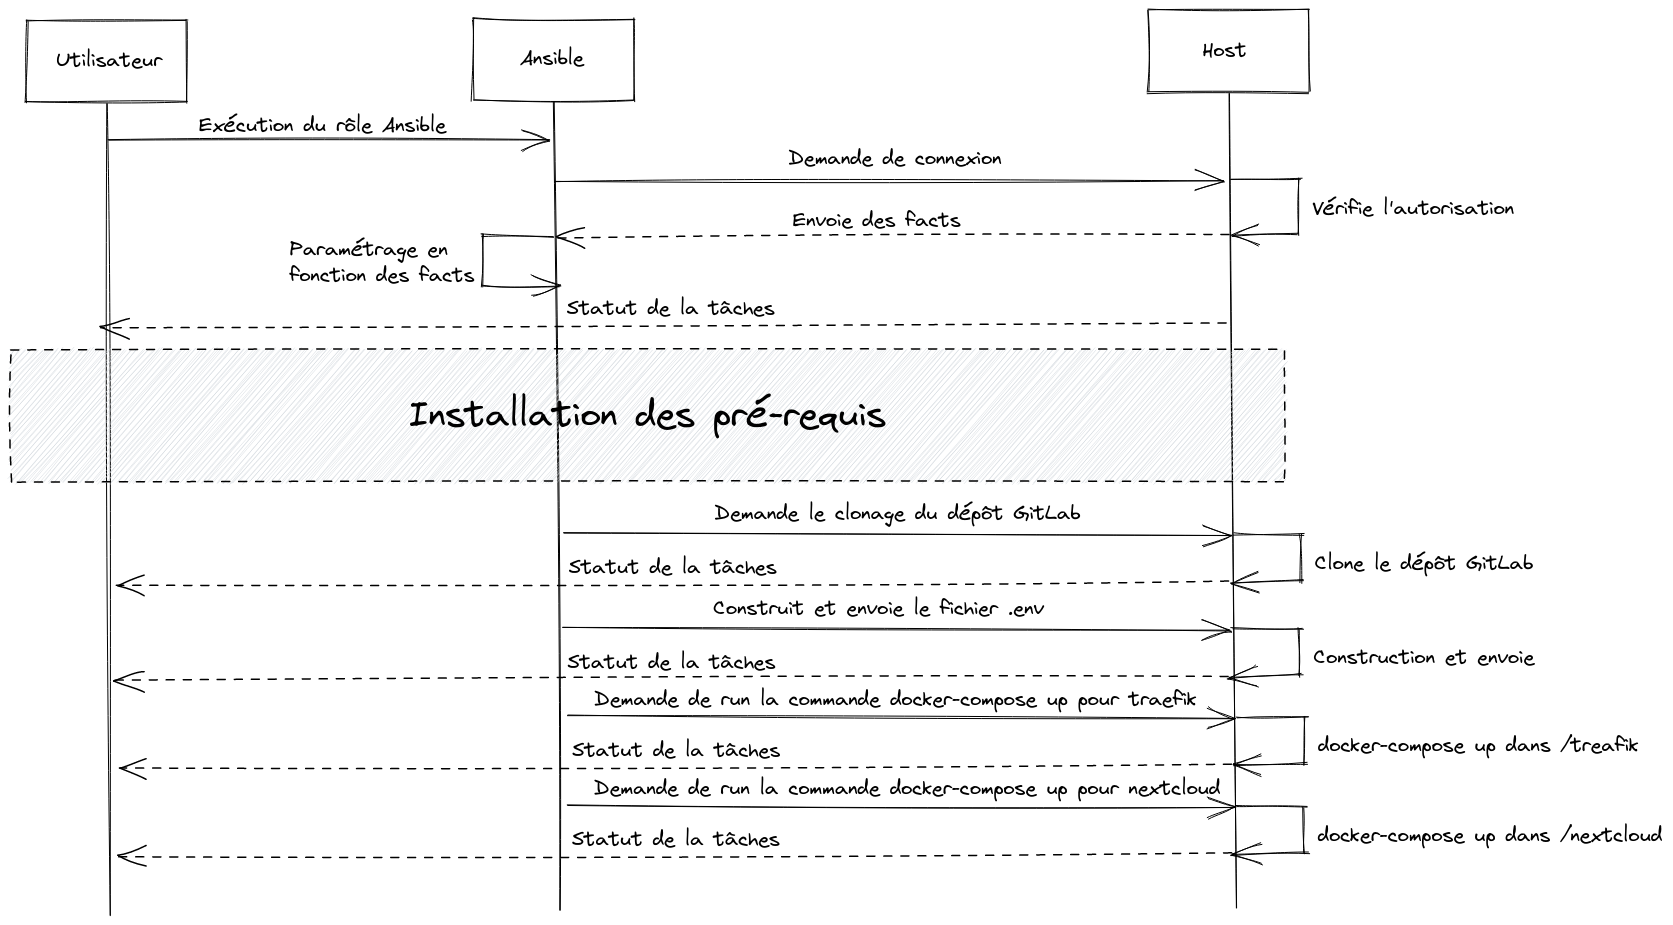
\includegraphics[width=\textwidth]{src/ansible_nextcloud.png}
    \caption{Diagramme de séquences des tâches Ansible lors de l'installation de Nextcloud}
    \label{fig:nextcloud_ansible}
\end{figure}

\subsubsection{Conclusion}
Lorsqu'une personne souhaite installer une nouvelle instance, il lui suffit de télécharger le dépôt GitLab et éditer la partie inventaire et vault puis de push ses modifications. 
Ensuite, dans Ansible AWX, il ajoute les ressources dont un inventaire, un script d'inventaire, deux informations d'identification et un modèle. 
Enfin, il exécute le modèles, ce qui lance l'installation de l'application.

Dans le cadre d'une installation, il aurait été possible de se limiter à la partie avec les fichiers docker-compose, sans se servir d'AWX. 
Cependant, AWX est particulièrement intéressant dans le maintien à jours des différentes instances. 
En effet, depuis AWX, en allant sur le projet \verb|nextcloud|, on peut y visualiser l'ensemble des ressources liées.

Cela fait donc office de listing de l'ensemble des instances nextcloud installé. 
Si la version d'un composant de nextcloud évolue, il suffit alors de modifier l'inventaire de chacun des modèles.

Ajouté à cela, on assure une installation homogène du produit. 
Dans le cas d'astreinte, on sait où trouver les ressources de l'application directement et ceux peu importe le Nextcloud sur lequel il faut intervenir.

De plus, il arrive souvent de laisser le fichier \verb|.env| directement sur la machine, ce qui est à éviter. 
Avec l'installation actuelle, le fichier \verb|.env| est généré, utilisé puis supprimé. 
Pour l'administration, l'ensemble des sysadmins enregistrent les mots de passes des vaults dans l'application Bitwarden, ce qui leurs permets dans tous les cas de récupéré les accès à une base de données par exemple.

\newpage
\subsection{Proxmox}
\subsubsection{Rappel}
\noindent%
\begin{minipage}{.7\textwidth}%
Proxmox est une plate-forme open-source complète pour la virtualisation d'entreprise. 
Grâce à l'interface Web intégrée, nous pouvons facilement gérer les machines virtuelles et les conteneurs, le stockage défini par logiciel, la mise en réseau, le clustering haute disponibilité et plusieurs outils prêts à l'emploi sur une seule solution.

\end{minipage}%
\hfill
\begin{minipage}{.3\textwidth}%
\begin{center}

\includegraphics[width=0.5\textwidth]{src/proxmox.JPG}
\end{center}
\end{minipage}% \\


\subsubsection{Objectif}
Les datacenters de Rennes et Tours utilisent une plate-forme de virtualisation nommé Proxmox. 
L'objectif est de mettre en oeuvre la même plate-forme de virtualisation à Angers pour que celle-ci puisse servir principalement à des tests. 
Pour cela, 3 serveurs sont disponibles afin de faire un cluster à 3 noeuds.

\subsubsection{Matériel}
Dans un premier temps, j'ai ajouté une carte fibre 10G pour ajouter une interface supplémentaire au serveur. 
Cette interface est destiné à faire transiter du traffic réseau ayant besoin de plus de débit qu'une simple interface 1G. 
L'interface 1G quant à elle sert à l'administration du serveur.
Dans un second temps, j'ai racké les serveurs dans une baies. 
Cela revient à positionner les différentes serveurs dans des tiroirs fixés.
Enfin, j'ai formaté l'ensemble des disques durs.
 Dans chacun serveur, un disque est réservé à l'installation du système d'exploitation et les autres servent au stockage des machines virtuelles.

\subsubsection{Logiciel}
\paragraph{Image}
Le système d'exploitation de Proxmox s'installe à partir d'un fichier ISO. Celui-ci est basé sur une image Debian. 
J'ai installé une version Proxmox VE 7.0 basé sur l'image Debian 11 nommé Bullseye à partir d'un disque dur externe IODD directement bootable. 
Cela permet de ne pas avoir à créer une clé Bootable dédié à cela.

\paragraph{Réseau}
Depuis l'interface graphique, j'ai configuré la partie DNS sur le DNS interne et changé l'adresse IP sur un réseau en 192.168.22.0/23. 
Le DHCP interne attribue par défaut des adresses sur le réseau 192.168.23.0/22.

Une fois cette étape terminée, les interfaces web de Proxmox sont disponibles à l'adresse IP configurée. 
Sur le DNS interne j'ai créé 3 enregistrements pour avoir les noms de domaines \verb|an-virt-pmx-1|, \verb|an-virt-pmx-2| et \verb|an-virt-pmx-3| pour chacun des noeuds.

\paragraph{Regroupement en cluster}
Depuis l'interface graphique, dans la section cluster, j'ai créé un cluster en lui donnant un nom et un réseau. Il se nomme \verb|an-virt-pmx|.
Ensuite, afin d'ajouter les 2 noeuds restant, j'ai récupéré le token d'identification du cluster, puis je me suis connecté sur chacun des noeuds. 
Sur chacun d'entres-eux, j'ai spécifié :
\begin{itemize}
    \item L'adresse IP du cluster, soit l'adresse IP d'\verb|an-virt-pmx-1|.
    \item Le token d'identification.
\end{itemize}

A partir de cette étape, depuis l'interface graphique de n'importe quel noeud Proxmox, l'ensemble des noeuds sont visibles et accessibles.

\begin{figure}
    \centering
        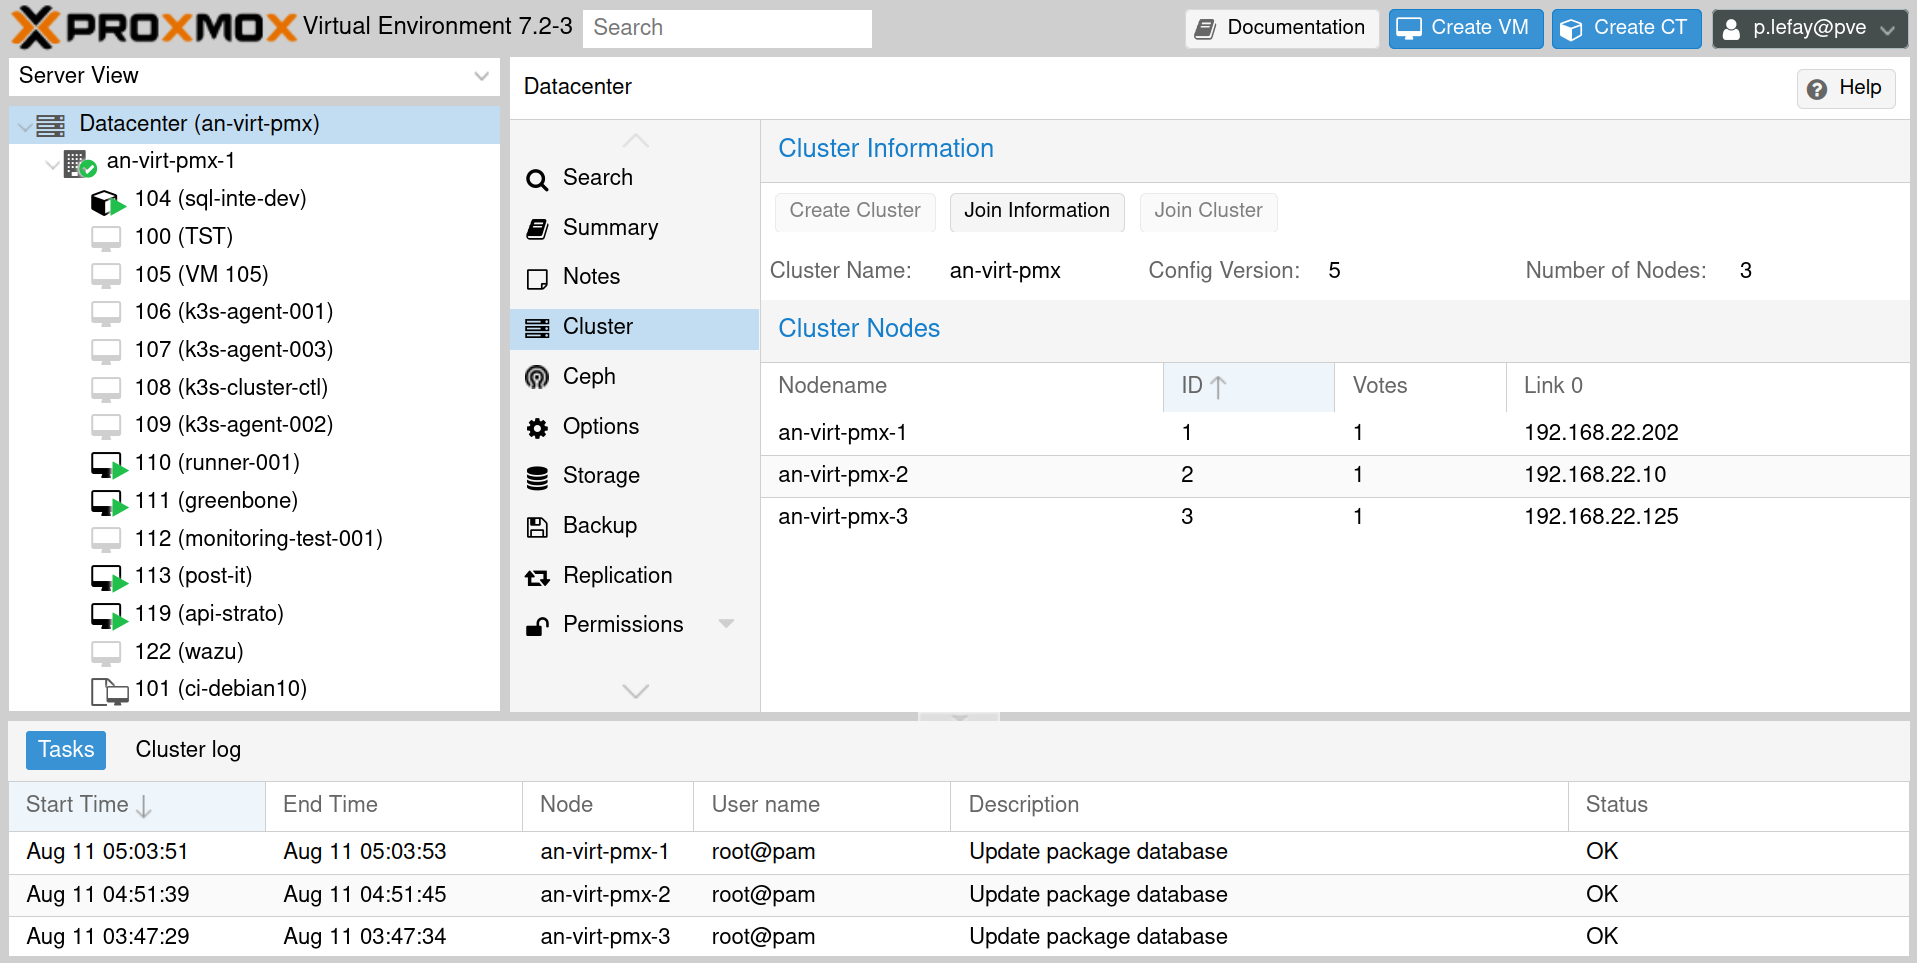
\includegraphics[width=\textwidth]{src/proxmox_interface.png}
    \caption{Interface du cluster Proxmox an-virt-pmx}
    \label{fig:proxmox_virt1}
\end{figure}

\paragraph{OSDS et manager}


\paragraph{Stockage}
J'ai créé un stockage CephFS afin d'y déposer l'ensemble des ISO qui pourraient être utiles. 
On y trouve différentes images pour Ubuntu, Debian, Fedora, CentOS et RockyLinux.

\newpage
\subsection{Projet Dehon} \label{dehon}
\subsubsection{Objectif}

Le groupe Dehon met en oeuvre un dispositif permettant la détection de fuite sur les installations frigorifiques. 
Un Détecteur de Niveau Intelligent (DNI) est donc installé sur chacune des installations frigorifique afin de détecter les fuites par méthodes de mesures indirectes.
Chaque DNI est également connecté au système de l'entreprise et les données sont remontées sur une plate-forme centralisée et consultable via un portail web. 

Une évolution des réglementation impose aux détenteurs d'installations frigorifiques de justifier d'un contrôle continu de leurs installations et de pouvoir présenter l'ensemble des vérifications ainsi que les opérations d'entretien effectuées.

L'objectif est donc de mettre en place une plateforme cloud pour centraliser l'exploitation de l'ensemble des DNI et proposer une offre de service complète de suivi et d'expertise en temps réel des installations frigorifiques.

J'ai travailler à la réalisation de cette infrastructure avec 2 autres administrateurs systèmes.

\subsubsection{Installation matériel}
Pour des raisons de disponibilité, l'infrastructure du projet se trouve sur 3 sites :
\begin{itemize}
    \item \textbf{virt2} : Proxmox de Tours à Cyrès sur lequel se trouve un premier cluster Kubernetes.
    \item \textbf{cogent} : Proxmox de Tours à Cogent sur lequel se trouve un répliqua du premier cluster de virt2.
    \item \textbf{virt1} : Proxmox de Rennes sur lequel se trouve un arbiter MongoDB. 
\end{itemize}

\newpage
En voici un schéma :
\begin{figure}
    \centering
        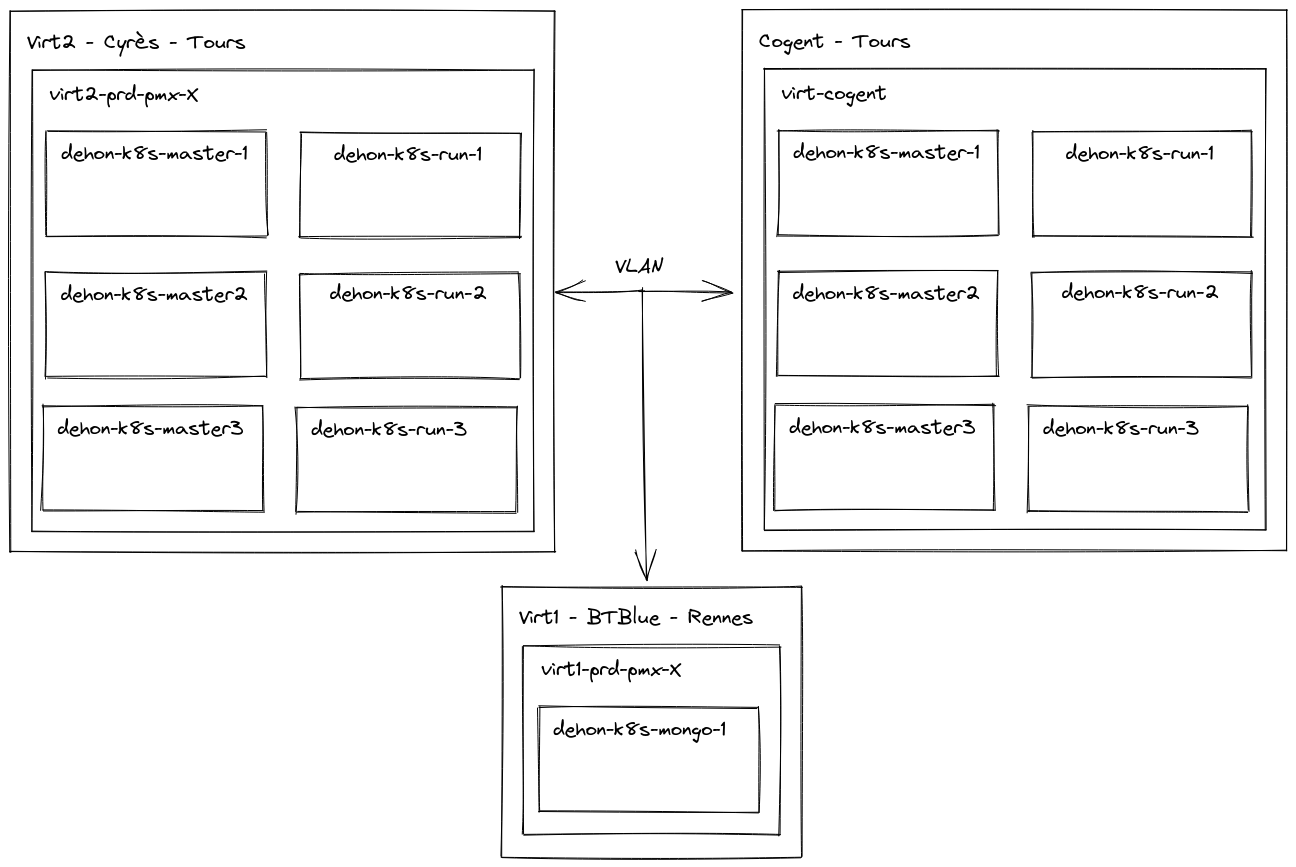
\includegraphics[width=\textwidth]{src/Dehon1.png}
    \caption{Infrastructure sur 3 sites physique du projet Dehon}
    \label{fig:dehon1}
\end{figure}

Les serveurs étaient déjà mis en place pour virt1 et virt2. 
Il a cependant fallu aller sur Tours chez cogent pour y installer une machine. 
Cette machine contient un unique cluster proxmox. 
Il a ensuite fallu relier les centres de Cogent et Cyrès. 
La distance entre les 2 bâtiments est d'environ 2 km. Une fibre noir, soit une fibre optique par encore activée à préalablement était installé par le personnel de Cyrès.

\subsubsection{Création des cluster de machines physiques avec proxmox et  terraform}
Nous avons commencé par developper l'infrastructure sur virt2. Nous nous sommes servis de terraform pour deployer les machinnes virtuelles sur le cluster. 
Nous avons donc 9 machines :

\begin{itemize}
    \item 3 machines virtuelles destinée a etre les masters. 
    Dans le conception de kubernetes, ces machines vont etre les cerveaux du cluster.
     c'est sur ces machines que des composant de kuberne vont permettre l'orchestration de runner.
    \item 3 machines virtuelle destinée a etre les workers. 
    Ces 3 machines vont etre celles qui supportent la charge de travail dans le cluster.
    \item 2 machines virtuelle en tant que proxy. 
    Elles seront le point d'entree de l'infrastructure. 
    \item 1 machines virtuelle pour le stockage. 
    L'ensemble du cluster utilisera un stockage partagé.
\end{itemize}

la denomination de ces machines est réfléchie afin d'identifier le client, le role et le nombre de chaque composant. 
Ces noms sont visibles sur le schema de l'infrastructure.

Avec Terragorm on declare dans un premier un format de machines virtuelle dans lequel on va attribuer des valeurs communes. 
Cela est dans notre cas par exemple le numero de vlan, le nom du client, les clées SSH a autorisées etc. 
La configurassions est par la suite appliquée a un template cloud\_init deja present sur les clusters.

Ensuite, on declare des modules specifique. par exemple, etant donne que les master sont identiques et au nombre de 3, on va declarer que l'on souhaite 3 machines master, que chacune aura 50 Gb de Ram, 4 CPU etc. 

une fois les fichiers de configuration terminé, on initialiser terraform pour lui specifier son etat, ses providers 

Ensuite, on lance une "planification". c'est a dire que l'on va lancer la commande "terraform plan"

\subsubsection{Installation du clusters Kubernetes via Kubespray}
\subsubsection{Configuration de proxy avec vip}
\subsubsection{IngressController, Certmanager, namespace, rancher rke}
\subsubsection{Stockage}
\subsubsection{Autres éléments}
Ex : mongo arbiter

\newpage
\subsection{Actualisation et mise en oeuvre de la procédure d'arrivée}
\subsubsection{Objectif}
Formaliser le besoin afin de rendre l'arrivée d'une nouvelle personne plus fluide et simple
\subsubsection{Description}
\subsubsection{Documentation}
\subsubsection{Groupe de Travail Embarquement}


\newpage
\subsection{Bilan}

\newpage
\section{Bilan personnel}


\newpage
\section{Annexes}
\subsection*{Les 16 thématiques de sécurité}
\begin{table}[!ht]
    \newcolumntype{M}[1]{>{\raggedright}m{#1}}
    % \center
    \begin{tabular}{|c|M{4cm}|M{11.5cm}|}
        \hline
        N° & \begin{center} Thèmes \end{center} & \begin{center}
            Description
        \end{center} 
        \tabularnewline
        
        \hline
        1 & Politique de l'information et gestion du risque & Il s'agit d'assurer l'utilisation de logiciels stables avec des suivi de correctifs. 
        De la documentation approuvée par la direction doit être rédigée afin d'assurer l'évolution du SI en matière de sécurité.
        \tabularnewline
        
        \hline
        2 & Organisation  de la sécurité de l'information & La sécurité de l'information doit être documentée en spécifiant les acteurs principaux sur chacun des domaines : développement applicatif, infrastructure, RGPD etc.
        \tabularnewline
        
        \hline
        3 & Sécurité des ressources humaines & L'exploitation d'un SI passant par ses utilisateurs, ils sont une sources indéniables de faille possible. 
        Les employés doivent être formés à la sécurité du SI et avoir accès en permanence à des documentations rappelant les règles de sécurités à appliquer. 
        \tabularnewline
        
        \hline
        4 & Gestion des actifs & Le matériel du personnel ainsi que toutes autres machines sur lesquelles reposent l'exploitation du SI doit être inventorié.
        \tabularnewline
        
        \hline
        5 & Contrôle d'accès et gestion des identités & L'utilisation du SI doit se faire de manière à pouvoir en tout temps identifier l'identité d'une personne l'exploitant. 
        Même si cela peut être contraignant dans l'exploitation, il n'est pas question d'ouvrir les accès à une ressources si la personne n'en a pas besoin. 
        L'ajout, la modification ou la suppression d'un accès quel-qu'il soit doit être documenté et archivé afin d'assurer un suivi.
        \tabularnewline

        \hline
        6 & Cryptologie & Des mécanismes cryptographique sécurisés doivent être employés lors de l'utilisation de protocoles tels que TLS, IPsec ou SSH.
        \tabularnewline
        
        \hline
        7 & Sécurité physique et environnementale & La sécurité des logicielles n'est pas suffisante. 
        Un aspect réglementaire oblige le découpage de zone d'accès aux différentes bâtiments. 
        Des mécanismes contre les sinistres tels que des inondations, coupures d'électricité ou incendie doivent permettre la continuité de l'activité.
        \tabularnewline

        \hline
        8 & Sécurité liée à l'exploitation & Il a de nombreuses règles lié à l'exploitation. 
        Celles-ci sont généralement liées aux autres sections du PSSI avec une prise en compte par exemple de l'exploitation de données sensibles, l'accès aux ressources informatiques, le nomadisme etc.
        \tabularnewline
        \hline
\end{tabular}
\caption{Les 16 thématiques de sécurité - Partie 1}
\label{tab:16thematiques1}
\end{table}

\newpage
\begin{table}[!ht]
    \newcolumntype{M}[1]{>{\raggedright}m{#1}}
    \center
    \begin{tabular}{|c|M{4cm}|M{11.5cm}|}
        \hline
        N° & Thèmes & \begin{center}
            Description
        \end{center} 
        \tabularnewline
        \hline
        9 & Sécurité des communications et réseau & Les différents équipements réseaux nécessite des configurations supplémentaires. 
        Cela concerne les différentes réseaux Wifi, Ethernet ainsi que les accès aux ressources distantes. 
        Des mécanismes de surveillance sur le SI doivent permettre la mise en avant d'une activité non-autorisée.
        \tabularnewline

        \hline
        10 & Acquisition, développement et maintenance des systèmes & Une des tâches les plus importante et pour autant ardue concerne la maintenance du système existant. 
        Il s'agit de garder les systèmes à des niveaux de sécurité satisfaisant sans impacter son exploitation. 
        Cela nécessite une vision en temps réel de l'état de l'infrastructure.
        \tabularnewline

        \hline
        11 & Relations avec les tiers & L'ouverture d'accès aux tiers sur des ressources du SI nécessite des procédures et documentations engageant la responsabilité des tiers en cas de faille. 
        Il est nécessaire de maintenir un listing des tiers et des ressources auxquels ils sont accès.
        \tabularnewline

        \hline
        12 & Gestion des incidents liés à la sécurité de l'information & De la documentation doit permettre l'évaluation rapide du niveau de criticité d'un incident. 
        Cette même documentation doit ensuite établir les acteurs à contacter : RSSI, DG, client etc.
        \tabularnewline

        \hline
        13 & Continuité d'activité & Le Plan de Continuité d'Activité (PCA), et le Plan de Reprise d'Activité (PRA) doivent prendre en comptes différents cas de figures afin d'assurer un maintien de l'activité en cas de sinistre.
        \tabularnewline

        \hline
        14 & Conformité & L'aspect conformité impose d'être en mesure d'assurer l'harmonisation des systèmes entre ce qui est prévu et effectif.
        \tabularnewline

        \hline
        15 & Poste de travail & Le développement du télé-travail nécessite de porter une attention particulière aux personnes en distanciel. 
        Leurs ordinateurs sont à configurer en conséquence.
        \tabularnewline

        \hline
        16 & Exigences supplémentaires & Les certifications imposent des aspects supplémentaire tels que la mise en oeuvre de convention de service avec les clients, l'obligation de stockage sur le territoire Européens etc.
        \tabularnewline

        \hline
\end{tabular}
\caption{Les 16 thématiques de sécurité - Partie 2}
\label{tab:16thematiques2}
\end{table}

\newpage
\subsection*{CV}
\begin{center}
    
\includegraphics[scale=0.9]{src/cv.png}
\end{center}

\newpage
\subsection*{Planning détaillé de la période d'alternance}
\begin{table}[!ht]
\newcolumntype{M}[1]{>{\raggedright}m{#1}}
\center
\begin{tabular}{|c|c|M{11.5cm}|}
    \hline
    N° & Semaine & \begin{center}
        Description
    \end{center} 
    \tabularnewline
    
    \hline
    36 & 06/09/21 - 12/09/21 & Découverte de l'entreprise et ses locaux. 
    Sensibilisation à l'accessibilité numérique et formation à la \gls{RGPD}. 
    Début de recherches documentaires basées sur les documentations de l'\gls{ANSSI}.
    \tabularnewline
    
    \hline
    37 & 13/09/21 - 19/09/21 & Pas de jours en entreprise cette semaine.
    \tabularnewline
    
    \hline
    38 & 20/09/21 - 26/09/21 & Poursuite des recherches documentaires. 
    Rendez-vous de mise au point sur l'ensemble de l'infrastructure technique du \gls{SI}. 
    Veille technologique sur les technologies/logiciels inconnues.
    \tabularnewline
    
    \hline
    39 & 27/09/21 - 03/10/21 & Mise en place d'un compte sur \gls{YesWeHack}. 
    Poursuite de la veille technologique. Ouverture des accès aux machines physiques et virtuelles.
    \tabularnewline
    
    \hline
    40 & 04/10/21 - 10/10/21 & Réunion avec le responsable le \gls{DPO} pour identifier les besoins de sécurité liés à la \gls{RGPD}. 
    \gls{POC} sur le logiciel \gls{Rudder} pour de la conformité d'infrastructure.
    \tabularnewline
    
    \hline
    41 & 11/10/21 - 17/10/21 & Ajout d'un agent et paramétrage de tests sur divers thématiques. 
    Réalisation d'un tableau d'audit pour l'ensemble des points mis en avant par la documentation de l'\gls{ANSSI}.
    \tabularnewline
    
    \hline
    42 & 18/10/21 - 24/10/21 & Pas de séance de \gls{PFE} cette semaine.
    \tabularnewline
    
    \hline
    43 & 25/10/21 - 31/10/21 & Poursuite de l'audit de l'état actuel de l'infrastructure à partir du tableau d'audit. 
    Ajout d'onglets plus spécifiques pour chacune des 15 sections du tableau.
    \tabularnewline
    
    \hline
    44 & 01/11/21 - 07/11/21 & Semaine complète excepté pour le lundi férié. 
    Amélioration du tableau d'audit et poursuite de celle-ci. 
    Veille sur les recommandations de l'ANSSI pour les protocoles \gls{IPsec}, \gls{TLS} et \gls{SSH}. 
    Rédaction du livre blanc de sécurité.
    \tabularnewline
    
    \hline
    45 & 08/11/21 - 14/11/21 & Séance de \gls{PFE} le vendredi mais congés posé ce jours là pour le pont avec le jeudi.
    \tabularnewline
    
    \hline
    46 & 15/11/21 - 21/11/21 & Début de la \gls{POC} \gls{Ansible CMDB} dans le but d'auditer les paquets et leurs versions.
    \tabularnewline
    
    \hline
    47 & 22/11/21 - 28/11/21 & Poursuite des travaux sur \gls{Ansible CMDB}. 
    Travaux sur la configuration de bornes {\gls{Wifi}}. Annulation des travaux pour cause de mauvaises configurations de ma part. 
    Visite médical et réunion de mi-avancement le vendredi.
    \tabularnewline
    
    \hline
\end{tabular}
\caption{Planning du travail effectué sur la période de d'alternance - Partie 1}
\end{table}

\newpage
\begin{table}[!htp]
    \newcolumntype{M}[1]{>{\raggedright}m{#1}}
    \center
    \begin{tabular}{|c|c|M{11.5cm}|}
        
        \hline
        48 & 29/11/21 - 05/12/21 & Fin des travaux sur \gls{Ansible CMDB} et rédaction du \gls{PSSI}.
        \tabularnewline
        
        \hline
        49 & 06/12/21 - 12/12/21 & Avancement sur le {\gls{POC}} Ansible. 
        Mise en place de règles basées sur les facts. 
        Mise au propre du compte rendu et établissement des éléments à auditer.
        \tabularnewline

        \hline
        50 & 13/12/21 - 19/11/21 & Avancement le \gls{PSSI}. 
        Réunion de présentation final de la \gls{POC} \gls{Ansible CMDB}. 
        Nouvelle \gls{POC} sur Rudder pour reproduire une conformité similaire à \gls{Ansible CMDB}.
        \tabularnewline
        
        \hline
        51 & 20/12/21 - 26/12/21 & Semaine complète en entreprise excepté le vendredi pour congé de Noël. 
        Avancement sur le \gls{PSSI}. Présentation bilan moral et financier de l'entreprise sur l'année 2020. 
        Vision sur les objectifs de 2022. Premier ticket client réalisé.
        \tabularnewline
        
        \hline
        52 & 27/12/21 - 02/01/22 & Congés pour Noël.
        \tabularnewline
        
        \hline
        1 & 03/01/22 - 09/01/22 & Poursuite des travaux sur la reprise du \gls{PSSI} pour le faire correspondre au tableau de suivi d'audit. 
        Intervention et découverte du datacenter de Rennes. 
        \tabularnewline
        \hline
        2 & 10/01/22 - 16/02/22 & Avancement sur le \gls{PSSI}, démonstration à un collégien du travail d'administrateur système avec l'installation d'un \gls{LAMP}. 
        Préparation de la soutenance de fin de \gls{PFE}.
        \tabularnewline
        
        \hline
        3 & 17/01/22 - 23/01/22 & Soutenance de \gls{PFE}. 
        Pas de journées en entreprise.
        \tabularnewline
        
        \hline
        4 & 24/01/22 - 30/01/22 & Pas de journées en entreprise.
        \tabularnewline   
    \hline
\end{tabular}
\caption{Planning du travail effectué sur la période de d'alternance - Partie 2}
\end{table}


\newpage
\subsection*{Planning détaillé de la période de stage}
\begin{table}[!ht]
\newcolumntype{M}[1]{>{\raggedright}m{#1}}
\center
\begin{tabular}{|c|c|M{11.5cm}|}
    \hline
    N° & Semaine & \begin{center}
        Description
    \end{center} 
    \tabularnewline    
    \hline
    9 & 28/02/22 - 06/03/22 & Installation d'un serveur de \gls{CVE}. 
    Ajout de l'import des logiciels à \gls{GLPI}. 
    Configuration d' \gls{OCSInventory} pour prendre en compte les rapports de \gls{CVE}. 
    Configuration de l'ordinateur pour un développeur. 
    Mise en place d'un scan \gls{SNMP} rattaché à \gls{GLPI} et \gls{OCSInventory}. 
    Installation de \gls{NocoDB} avec sauvegarde \gls{SQL} de la base de données de \gls{Redmine}. 
    Reprise de la documentation technique liée aux \gls{datacenters}.
    \tabularnewline
    
    \hline
    10 & 07/03/22 - 13/03/22 & Configuration du serveur \gls{OCSInventory} en \gls{HTTPS} avec un certificat auto-signé pour pouvoir effectuer des scans \gls{SNMP} à partir d'agent spécifique. 
    Modifications du comportement de l'agent vers \gls{HTTPS} avec activation \gls{SSL}. 
    Poursuite des travaux sur la documentation technique et rédaction du rapport de stage. 
    Maintenance d'un ordinateur qui ne boot plus : changements depuis un disque externe pour revenir sur un ancien noyau Linux mais problème lié au driver graphique. 
    Installation d'une carte d'extension 10G sur un noeud \gls{Proxmox}. 
    Installation d'un \gls{LimeSurvey} de test en conteneur pour un client. 
    Installation d'un noeud \gls{Proxmox} puis début de configuration d'un \gls{cluster} \gls{Ceph}.
    \tabularnewline
    
    \hline
    11 & 14/03/22 - 20/03/22 & Réunion de lancement d'audit de sécurité avec la société Cogiceo. 
    Poursuite de la configuration du \gls{cluster} \gls{Ceph}, ajout des \gls{OSD}.
    Configuration en pause pour le moment en attendant de faire la conception des pools et storages. 
    Modification des configurations \gls{DHCP} de façon à ce que tout le monde soit sur une adresse \gls{IP} en 22. 
    Reprise de la configuration des règles \gls{GLPI} avant l'ajout de tous les périphériques. 
    Installation de NetData pour vérifier le fonctionnement d'une machine défectueuse. 
    Installation et configuration d'un nouveau noeud \gls{Proxmox} ajouté au \gls{cluster} de test. 
    Fin de paramétrage de \gls{GLPI} avant d'ajouter l'ensemble du matériel du personnel.
    \tabularnewline


\hline
\end{tabular}
\caption{Planning du travail effectué sur la période de stage - Partie 1}
\end{table}

\newpage
\begin{table}[!ht]
\newcolumntype{M}[1]{>{\raggedright}m{#1}}
\center
\begin{tabular}{|c|c|M{11.5cm}|}
    \hline
    N° & Semaine & \begin{center}
        Description
    \end{center} 
    \tabularnewline

    \hline
    13 & 28/03/28 - 03/04/22 & Fin des installations pour l'audit de sécurité avec l'installation de \gls{Passhport}. 
    Lancement de l'installation des agents \gls{OCSInventory} sur l'ensemble des ordinateurs du personnel. 
    Test de l'application \gls{Wazuh} pour du monitoring de sécurité. 
    Préparation de l'environnement local pour l'exécution de scripts \gls{Ansible} en production. 
    Correction du script \gls{Ansible} pour la prise en compte des différences entre \gls{CentOS} 7 et 8, avec spécification pour \gls{Rocky}, \gls{Alma} etc. 
    Ajout de l'agent \gls{OCSInventory} sur toutes les machines du datacenter d'Angers.
    \tabularnewline
    
    \hline
    14 & 04/04/22 - 10/04/22 & Fin de l'installation des agents \gls{OCSInventory} pour les machines du datacenter d'Angers. 
    Début de l'installation des agents pour le datacenter de Tours. Poursuite des travaux sur la documentation. 
    Installation pour un client d'un \gls{Nextcloud}/\gls{Collabora} pour un client sur le datacenter de Rennes via Docker-compose.  
    \tabularnewline
    
    \hline
    15 & 11/04/22 - 17/04/22 & Ajout de l'agent \gls{OCSInventory} sur toutes les machines du datacenters de Rennes. 
    Installation et configuration de \gls{Wazuh} pour réaliser un audit automatisés de l'infrastructure.
    \tabularnewline
    
    \hline
    16 & 18/04/22 - 24/04/22 & Intervention au datacenter pour le changement d'un serveur. Poursuite des travaux sur la documentation. 
    Poursuite des travaux avec \gls{Wazuh}. Installation d'un \gls{cluster} \gls{Kubernetes} à 2 noeuds pour pouvoir y faire de la veille technologique. 
    Mise en place du stockage du \gls{cluster} \gls{Kubernetes}. 
    Préparation d'un ordinateur pour un nouvel employé.
    \tabularnewline
    
    \hline
    17 & 25/04/22 - 01/05/22 &  Poursuite de la veille sur \gls{Kubernetes}. Début des travaux pour auditer les ressources des datacenters. 
    L'idée est d'avoir un outil permettant de contrôler que ce qui est vendu au client est bien respecté en matière de ressources.
    \tabularnewline
    
    \hline
    18 & 02/05/22 - 08/05/22 &  Mise à jour de l'inventaire \gls{Ansible} qui avait des défauts dans sa constructions. 
    Modifications de différents problèmes empêchant l'installation des agents \gls{OCSInventory}. 
    Installation d'une nouvelle instance d'un site internet pour réaliser des \gls{webinaires}.
    \tabularnewline
    
    \hline
\end{tabular}
\caption{Planning du travail effectué sur la période de stage - Partie 2}
\end{table}

\newpage
\begin{table}[!ht]
\newcolumntype{M}[1]{>{\raggedright}m{#1}}
\center
\begin{tabular}{|c|c|M{11.5cm}|}
    \hline
    N° & Semaine & \begin{center}
        Description
    \end{center} 
    \tabularnewline

    \hline
    19 & 09/05/22 - 15/05/22 &  Mise à jours de l'une des instances de \gls{webinaires}. 
    Modification des scripts Perl/Bash pour récupérer les \gls{vhosts} des machines que ce soit pour des vhosts hébergés sous \gls{Docker}/\gls{Nginx} ou \gls{Apache}. 
    Mise en place d'une \gls{plate-forme web}\gls{Peertube} pour faire de l'hébergement vidéo et des lives. 
    Installation d'un 2nd \gls{bastion SSH} (\gls{passhport}) destiné à être un slave du 1er afin d'y exécuter des \gls{playbooks} \gls{Ansible} globaux sans impact sur l'utilisation des autres utilisateurs. 
    Création de la 2nd base de données en \gls{Master/Slave} sur \gls{Mariadb}.
    \tabularnewline

    \hline
    20 & 16/05/22 - 22/05/22 & Fin de l'installation du 2nd \gls{bastion SSH} (\gls{passhport}). 
    Ré-exécution des \gls{playbooks} \gls{Ansible} d'installation d'agent \gls{OCSInventory} afin de mettre à jours l'ensemble des \gls{vhosts}. 
    En congé le vendredi 20. Début des mise à jours des instances \gls{BigBlueButton}
    \tabularnewline
    
    \hline
    21 & 23/05/22 - 29/05/22 & Poursuite de la ré-exécution des \gls{playbooks} \gls{Ansible} d'installation d'agent \gls{OCSInventory} afin de mettre à jours l'ensemble des \gls{vhosts}. 
    Poursuite des mise à jours des instances \gls{BigBlueButton}. 
    Congé le lundi 23, jeudi 26 et vendredi 27.
    \tabularnewline
    
    \hline
    22 & 30/05/22 - 05/06/22 & Fin de la ré-exécution des \gls{playbooks} \gls{Ansible} d'installation d'agent \gls{OCSInventory}. 
    Recherche d'une solution sans agent pour faire un état des lieux en matières de sécurité des différentes machines et automatiser la mise en oeuvre de correctif. 
    Les tests s'appliquent à  \gls{OpenSCAP}. 
    Rédaction d'un Plan d'Assurance de Sécurité dans le cadre d'une demande d'un client. 
    Poursuite des travaux sur la documentation du datacenter.
    \tabularnewline
    
    \hline
    23 & 06/06/22 - 12/06/22 & Installation d'une nouvelle instance \gls{Framemo}, sur un nom de domaine publique. 
    Poursuite des travaux sur \gls{OpenSCAP}. 
    Réunion de lancement pour un projet d'infrastructure pour Dehon. 
    Début des travaux sur le projet Dehon avec \gls{Terraform} pour la création des machines virtuelles.
    \tabularnewline
    
    \hline
    24 & 13/06/22 - 19/06/22 & Création des machines virtuelles pour le projet Dehon. 
    Création du \gls{cluster} \gls{Kubernetes} avec \gls{Calico} en \gls{CNI} sur les 6 précédentes machines virtuelles avec \gls{Kubespray}. 
    Installation d'un ordinateur portable pour un nouvel arrivant. 
    Poursuite des travaux sur \gls{OpenSCAP}.
    \tabularnewline
    



    \hline
\end{tabular}
\caption{Planning du travail effectué sur la période de stage - Partie 3}
\end{table}

\newpage
\begin{table}[!ht]
\newcolumntype{M}[1]{>{\raggedright}m{#1}}
\center
\begin{tabular}{|c|c|M{11.5cm}|}
    \hline
    N° & Semaine & \begin{center}
        Description
    \end{center} 
    \tabularnewline

    \hline
    25 & 20/06/22 - 26/06/22 & Poursuite des travaux sur \gls{OpenSCAP}. 
    Rédaction d'une documentation utilisateur sur la configuration de l'agenda \gls{Nextcloud} sur téléphone. 
    Début de recherches pour la mise en place d'un outil de scan du réseau. Rédaction du rapport de stage. 
    Intervention aux datacenters de Tours et Cogent. 
    Ticket client pour la configuration d'un agenda \gls{Nextcloud}.
    \tabularnewline

    \hline
    26 & 27/06/22 - 03/07/22 & Recherche et intervention pour planifiée pour les travaux sur \gls{Nextcloud}. 
    Poursuite des travaux sur Dehon avec le lancement des 2 \gls{Haproxy} avec \gls{vip}. 
    Configuration et test des configurations \gls{Haproxy}. 
    Mise en place sur Dehon des IngressController, CertManager, Namespaces et Rancher rke.
    \tabularnewline

    \hline
    27 & 04/07/22 - 10/07/22 & Mise en place sur Dehon de Rancher rke. 
    Rédaction de la documentation technique du projet Dehon sur le déploiement de l'ensemble du projet. 
    Journée Team Building au lac de Maine avec présentation du bilan du premier semestre de l'entreprise. 
    Mise en place des environnements/namespaces de prod/qualif/test avec \gls{Terraform} en passant l'\gls{API} de Rancher. 
    Installation de la machine de stockage avec Terraform. 
    Particularité devoir ajouter un second disque et donc recréer un module Terraform.
    \tabularnewline
    
    \hline
    28 & 11/07/22 - 17/07/22 & Déploiement de la machine Mongo Arbiter sur Rennes. 
    Configuration du service Mongo via Terraform pour une application sous Docker. 
    Installation via Terraform de 3 opérateurs percona pour les environnements de test, qualif et prod. 
    Installation de mongoarbiter via Ansible. 
    Congé le vendredi, pont de 4 jours.
    \tabularnewline
    
    \hline
    29 & 18/07/22 - 24/07/22 & Commandes pour les nouveaux arrivants. 
    Création de compte rancher depuis Terraform. 
    Déploiement de Loki lié à Grafana en tant que serveur de log pour l'ensemble du cluster. 
    Ajout de minio en serveur S3. Ajout de Velero-server pour les backups. 
    Fin de la mise à jours de la documentation pour les nouveaux arrivants. 
    Reprise de la partie backup pour un matomo de la région Normandie.
    \tabularnewline

    \hline
    30 & 25/07/22 - 31/07/22 & Installation d'un Nextcloud pour l'association AICLA. 
    Automatisation de l'installation des instances Nextcloud via Docker-compose, Ansible, AWX et Terraform.
    \tabularnewline
    
    \hline
    31 & 01/08/22 - 07/08/22 & Configuration d'un stockage CephFS sur le Proxmox d'Angers. 
    Accompagnement d'un client dans la configuration de son Nextcloud. Congés maladie pour Covid.
    \tabularnewline
    
    \hline    
\end{tabular}
\caption{Planning du travail effectué sur la période de stage - Partie 4}
\end{table}

\newpage
\subsection*{Bibliographie}
% Bibliography
\bibliographystyle{unsrt}
\nocite{*}
\bibliography{bibliography}


\newpage
\subsection*{Liste des figures}
\listoffigures

\newpage
\subsection*{Liste des tables}
\listoftables

\newpage
\subsection*{Acronymes et définition}
L'ensemble des acronymes et définition du glossaires proviennent de Wikipédia.
\glsaddall
\printglossaries

\end{document}